\documentclass[conference,compsoc]{IEEEtran}
% IEEE Symposium on Security and Privacy / Computer Society conference layout.
% The manuscript remains split across the original section files.
\IEEEoverridecommandlockouts

% Optional math commands from https://github.com/goodfeli/dlbook_notation.
%%%%% NEW MATH DEFINITIONS %%%%%

\usepackage{amsmath,amsfonts,bm}

% Mark sections of captions for referring to divisions of figures
\newcommand{\figleft}{{\em (Left)}}
\newcommand{\figcenter}{{\em (Center)}}
\newcommand{\figright}{{\em (Right)}}
\newcommand{\figtop}{{\em (Top)}}
\newcommand{\figbottom}{{\em (Bottom)}}
\newcommand{\captiona}{{\em (a)}}
\newcommand{\captionb}{{\em (b)}}
\newcommand{\captionc}{{\em (c)}}
\newcommand{\captiond}{{\em (d)}}

% Highlight a newly defined term
\newcommand{\newterm}[1]{{\bf #1}}


% Figure reference, lower-case.
\def\figref#1{figure~\ref{#1}}
% Figure reference, capital. For start of sentence
\def\Figref#1{Figure~\ref{#1}}
\def\twofigref#1#2{figures \ref{#1} and \ref{#2}}
\def\quadfigref#1#2#3#4{figures \ref{#1}, \ref{#2}, \ref{#3} and \ref{#4}}
% Section reference, lower-case.
\def\secref#1{section~\ref{#1}}
% Section reference, capital.
\def\Secref#1{Section~\ref{#1}}
% Reference to two sections.
\def\twosecrefs#1#2{sections \ref{#1} and \ref{#2}}
% Reference to three sections.
\def\secrefs#1#2#3{sections \ref{#1}, \ref{#2} and \ref{#3}}
% Reference to an equation, lower-case.
\def\eqref#1{equation~\ref{#1}}
% Reference to an equation, upper case
\def\Eqref#1{Equation~\ref{#1}}
% A raw reference to an equation---avoid using if possible
\def\plaineqref#1{\ref{#1}}
% Reference to a chapter, lower-case.
\def\chapref#1{chapter~\ref{#1}}
% Reference to an equation, upper case.
\def\Chapref#1{Chapter~\ref{#1}}
% Reference to a range of chapters
\def\rangechapref#1#2{chapters\ref{#1}--\ref{#2}}
% Reference to an algorithm, lower-case.
\def\algref#1{algorithm~\ref{#1}}
% Reference to an algorithm, upper case.
\def\Algref#1{Algorithm~\ref{#1}}
\def\twoalgref#1#2{algorithms \ref{#1} and \ref{#2}}
\def\Twoalgref#1#2{Algorithms \ref{#1} and \ref{#2}}
% Reference to a part, lower case
\def\partref#1{part~\ref{#1}}
% Reference to a part, upper case
\def\Partref#1{Part~\ref{#1}}
\def\twopartref#1#2{parts \ref{#1} and \ref{#2}}

\def\ceil#1{\lceil #1 \rceil}
\def\floor#1{\lfloor #1 \rfloor}
\def\1{\bm{1}}
\newcommand{\train}{\mathcal{D}}
\newcommand{\valid}{\mathcal{D_{\mathrm{valid}}}}
\newcommand{\test}{\mathcal{D_{\mathrm{test}}}}

\def\eps{{\epsilon}}


% Random variables
\def\reta{{\textnormal{$\eta$}}}
\def\ra{{\textnormal{a}}}
\def\rb{{\textnormal{b}}}
\def\rc{{\textnormal{c}}}
\def\rd{{\textnormal{d}}}
\def\re{{\textnormal{e}}}
\def\rf{{\textnormal{f}}}
\def\rg{{\textnormal{g}}}
\def\rh{{\textnormal{h}}}
\def\ri{{\textnormal{i}}}
\def\rj{{\textnormal{j}}}
\def\rk{{\textnormal{k}}}
\def\rl{{\textnormal{l}}}
% rm is already a command, just don't name any random variables m
\def\rn{{\textnormal{n}}}
\def\ro{{\textnormal{o}}}
\def\rp{{\textnormal{p}}}
\def\rq{{\textnormal{q}}}
\def\rr{{\textnormal{r}}}
\def\rs{{\textnormal{s}}}
\def\rt{{\textnormal{t}}}
\def\ru{{\textnormal{u}}}
\def\rv{{\textnormal{v}}}
\def\rw{{\textnormal{w}}}
\def\rx{{\textnormal{x}}}
\def\ry{{\textnormal{y}}}
\def\rz{{\textnormal{z}}}

% Random vectors
\def\rvepsilon{{\mathbf{\epsilon}}}
\def\rvtheta{{\mathbf{\theta}}}
\def\rva{{\mathbf{a}}}
\def\rvb{{\mathbf{b}}}
\def\rvc{{\mathbf{c}}}
\def\rvd{{\mathbf{d}}}
\def\rve{{\mathbf{e}}}
\def\rvf{{\mathbf{f}}}
\def\rvg{{\mathbf{g}}}
\def\rvh{{\mathbf{h}}}
\def\rvu{{\mathbf{i}}}
\def\rvj{{\mathbf{j}}}
\def\rvk{{\mathbf{k}}}
\def\rvl{{\mathbf{l}}}
\def\rvm{{\mathbf{m}}}
\def\rvn{{\mathbf{n}}}
\def\rvo{{\mathbf{o}}}
\def\rvp{{\mathbf{p}}}
\def\rvq{{\mathbf{q}}}
\def\rvr{{\mathbf{r}}}
\def\rvs{{\mathbf{s}}}
\def\rvt{{\mathbf{t}}}
\def\rvu{{\mathbf{u}}}
\def\rvv{{\mathbf{v}}}
\def\rvw{{\mathbf{w}}}
\def\rvx{{\mathbf{x}}}
\def\rvy{{\mathbf{y}}}
\def\rvz{{\mathbf{z}}}

% Elements of random vectors
\def\erva{{\textnormal{a}}}
\def\ervb{{\textnormal{b}}}
\def\ervc{{\textnormal{c}}}
\def\ervd{{\textnormal{d}}}
\def\erve{{\textnormal{e}}}
\def\ervf{{\textnormal{f}}}
\def\ervg{{\textnormal{g}}}
\def\ervh{{\textnormal{h}}}
\def\ervi{{\textnormal{i}}}
\def\ervj{{\textnormal{j}}}
\def\ervk{{\textnormal{k}}}
\def\ervl{{\textnormal{l}}}
\def\ervm{{\textnormal{m}}}
\def\ervn{{\textnormal{n}}}
\def\ervo{{\textnormal{o}}}
\def\ervp{{\textnormal{p}}}
\def\ervq{{\textnormal{q}}}
\def\ervr{{\textnormal{r}}}
\def\ervs{{\textnormal{s}}}
\def\ervt{{\textnormal{t}}}
\def\ervu{{\textnormal{u}}}
\def\ervv{{\textnormal{v}}}
\def\ervw{{\textnormal{w}}}
\def\ervx{{\textnormal{x}}}
\def\ervy{{\textnormal{y}}}
\def\ervz{{\textnormal{z}}}

% Random matrices
\def\rmA{{\mathbf{A}}}
\def\rmB{{\mathbf{B}}}
\def\rmC{{\mathbf{C}}}
\def\rmD{{\mathbf{D}}}
\def\rmE{{\mathbf{E}}}
\def\rmF{{\mathbf{F}}}
\def\rmG{{\mathbf{G}}}
\def\rmH{{\mathbf{H}}}
\def\rmI{{\mathbf{I}}}
\def\rmJ{{\mathbf{J}}}
\def\rmK{{\mathbf{K}}}
\def\rmL{{\mathbf{L}}}
\def\rmM{{\mathbf{M}}}
\def\rmN{{\mathbf{N}}}
\def\rmO{{\mathbf{O}}}
\def\rmP{{\mathbf{P}}}
\def\rmQ{{\mathbf{Q}}}
\def\rmR{{\mathbf{R}}}
\def\rmS{{\mathbf{S}}}
\def\rmT{{\mathbf{T}}}
\def\rmU{{\mathbf{U}}}
\def\rmV{{\mathbf{V}}}
\def\rmW{{\mathbf{W}}}
\def\rmX{{\mathbf{X}}}
\def\rmY{{\mathbf{Y}}}
\def\rmZ{{\mathbf{Z}}}

% Elements of random matrices
\def\ermA{{\textnormal{A}}}
\def\ermB{{\textnormal{B}}}
\def\ermC{{\textnormal{C}}}
\def\ermD{{\textnormal{D}}}
\def\ermE{{\textnormal{E}}}
\def\ermF{{\textnormal{F}}}
\def\ermG{{\textnormal{G}}}
\def\ermH{{\textnormal{H}}}
\def\ermI{{\textnormal{I}}}
\def\ermJ{{\textnormal{J}}}
\def\ermK{{\textnormal{K}}}
\def\ermL{{\textnormal{L}}}
\def\ermM{{\textnormal{M}}}
\def\ermN{{\textnormal{N}}}
\def\ermO{{\textnormal{O}}}
\def\ermP{{\textnormal{P}}}
\def\ermQ{{\textnormal{Q}}}
\def\ermR{{\textnormal{R}}}
\def\ermS{{\textnormal{S}}}
\def\ermT{{\textnormal{T}}}
\def\ermU{{\textnormal{U}}}
\def\ermV{{\textnormal{V}}}
\def\ermW{{\textnormal{W}}}
\def\ermX{{\textnormal{X}}}
\def\ermY{{\textnormal{Y}}}
\def\ermZ{{\textnormal{Z}}}

% Vectors
\def\vzero{{\bm{0}}}
\def\vone{{\bm{1}}}
\def\vmu{{\bm{\mu}}}
\def\vtheta{{\bm{\theta}}}
\def\va{{\bm{a}}}
\def\vb{{\bm{b}}}
\def\vc{{\bm{c}}}
\def\vd{{\bm{d}}}
\def\ve{{\bm{e}}}
\def\vf{{\bm{f}}}
\def\vg{{\bm{g}}}
\def\vh{{\bm{h}}}
\def\vi{{\bm{i}}}
\def\vj{{\bm{j}}}
\def\vk{{\bm{k}}}
\def\vl{{\bm{l}}}
\def\vm{{\bm{m}}}
\def\vn{{\bm{n}}}
\def\vo{{\bm{o}}}
\def\vp{{\bm{p}}}
\def\vq{{\bm{q}}}
\def\vr{{\bm{r}}}
\def\vs{{\bm{s}}}
\def\vt{{\bm{t}}}
\def\vu{{\bm{u}}}
\def\vv{{\bm{v}}}
\def\vw{{\bm{w}}}
\def\vx{{\bm{x}}}
\def\vy{{\bm{y}}}
\def\vz{{\bm{z}}}

% Elements of vectors
\def\evalpha{{\alpha}}
\def\evbeta{{\beta}}
\def\evepsilon{{\epsilon}}
\def\evlambda{{\lambda}}
\def\evomega{{\omega}}
\def\evmu{{\mu}}
\def\evpsi{{\psi}}
\def\evsigma{{\sigma}}
\def\evtheta{{\theta}}
\def\eva{{a}}
\def\evb{{b}}
\def\evc{{c}}
\def\evd{{d}}
\def\eve{{e}}
\def\evf{{f}}
\def\evg{{g}}
\def\evh{{h}}
\def\evi{{i}}
\def\evj{{j}}
\def\evk{{k}}
\def\evl{{l}}
\def\evm{{m}}
\def\evn{{n}}
\def\evo{{o}}
\def\evp{{p}}
\def\evq{{q}}
\def\evr{{r}}
\def\evs{{s}}
\def\evt{{t}}
\def\evu{{u}}
\def\evv{{v}}
\def\evw{{w}}
\def\evx{{x}}
\def\evy{{y}}
\def\evz{{z}}

% Matrix
\def\mA{{\bm{A}}}
\def\mB{{\bm{B}}}
\def\mC{{\bm{C}}}
\def\mD{{\bm{D}}}
\def\mE{{\bm{E}}}
\def\mF{{\bm{F}}}
\def\mG{{\bm{G}}}
\def\mH{{\bm{H}}}
\def\mI{{\bm{I}}}
\def\mJ{{\bm{J}}}
\def\mK{{\bm{K}}}
\def\mL{{\bm{L}}}
\def\mM{{\bm{M}}}
\def\mN{{\bm{N}}}
\def\mO{{\bm{O}}}
\def\mP{{\bm{P}}}
\def\mQ{{\bm{Q}}}
\def\mR{{\bm{R}}}
\def\mS{{\bm{S}}}
\def\mT{{\bm{T}}}
\def\mU{{\bm{U}}}
\def\mV{{\bm{V}}}
\def\mW{{\bm{W}}}
\def\mX{{\bm{X}}}
\def\mY{{\bm{Y}}}
\def\mZ{{\bm{Z}}}
\def\mBeta{{\bm{\beta}}}
\def\mPhi{{\bm{\Phi}}}
\def\mLambda{{\bm{\Lambda}}}
\def\mSigma{{\bm{\Sigma}}}

% Tensor
\DeclareMathAlphabet{\mathsfit}{\encodingdefault}{\sfdefault}{m}{sl}
\SetMathAlphabet{\mathsfit}{bold}{\encodingdefault}{\sfdefault}{bx}{n}
\newcommand{\tens}[1]{\bm{\mathsfit{#1}}}
\def\tA{{\tens{A}}}
\def\tB{{\tens{B}}}
\def\tC{{\tens{C}}}
\def\tD{{\tens{D}}}
\def\tE{{\tens{E}}}
\def\tF{{\tens{F}}}
\def\tG{{\tens{G}}}
\def\tH{{\tens{H}}}
\def\tI{{\tens{I}}}
\def\tJ{{\tens{J}}}
\def\tK{{\tens{K}}}
\def\tL{{\tens{L}}}
\def\tM{{\tens{M}}}
\def\tN{{\tens{N}}}
\def\tO{{\tens{O}}}
\def\tP{{\tens{P}}}
\def\tQ{{\tens{Q}}}
\def\tR{{\tens{R}}}
\def\tS{{\tens{S}}}
\def\tT{{\tens{T}}}
\def\tU{{\tens{U}}}
\def\tV{{\tens{V}}}
\def\tW{{\tens{W}}}
\def\tX{{\tens{X}}}
\def\tY{{\tens{Y}}}
\def\tZ{{\tens{Z}}}


% Graph
\def\gA{{\mathcal{A}}}
\def\gB{{\mathcal{B}}}
\def\gC{{\mathcal{C}}}
\def\gD{{\mathcal{D}}}
\def\gE{{\mathcal{E}}}
\def\gF{{\mathcal{F}}}
\def\gG{{\mathcal{G}}}
\def\gH{{\mathcal{H}}}
\def\gI{{\mathcal{I}}}
\def\gJ{{\mathcal{J}}}
\def\gK{{\mathcal{K}}}
\def\gL{{\mathcal{L}}}
\def\gM{{\mathcal{M}}}
\def\gN{{\mathcal{N}}}
\def\gO{{\mathcal{O}}}
\def\gP{{\mathcal{P}}}
\def\gQ{{\mathcal{Q}}}
\def\gR{{\mathcal{R}}}
\def\gS{{\mathcal{S}}}
\def\gT{{\mathcal{T}}}
\def\gU{{\mathcal{U}}}
\def\gV{{\mathcal{V}}}
\def\gW{{\mathcal{W}}}
\def\gX{{\mathcal{X}}}
\def\gY{{\mathcal{Y}}}
\def\gZ{{\mathcal{Z}}}

% Sets
\def\sA{{\mathbb{A}}}
\def\sB{{\mathbb{B}}}
\def\sC{{\mathbb{C}}}
\def\sD{{\mathbb{D}}}
% Don't use a set called E, because this would be the same as our symbol
% for expectation.
\def\sF{{\mathbb{F}}}
\def\sG{{\mathbb{G}}}
\def\sH{{\mathbb{H}}}
\def\sI{{\mathbb{I}}}
\def\sJ{{\mathbb{J}}}
\def\sK{{\mathbb{K}}}
\def\sL{{\mathbb{L}}}
\def\sM{{\mathbb{M}}}
\def\sN{{\mathbb{N}}}
\def\sO{{\mathbb{O}}}
\def\sP{{\mathbb{P}}}
\def\sQ{{\mathbb{Q}}}
\def\sR{{\mathbb{R}}}
\def\sS{{\mathbb{S}}}
\def\sT{{\mathbb{T}}}
\def\sU{{\mathbb{U}}}
\def\sV{{\mathbb{V}}}
\def\sW{{\mathbb{W}}}
\def\sX{{\mathbb{X}}}
\def\sY{{\mathbb{Y}}}
\def\sZ{{\mathbb{Z}}}

% Entries of a matrix
\def\emLambda{{\Lambda}}
\def\emA{{A}}
\def\emB{{B}}
\def\emC{{C}}
\def\emD{{D}}
\def\emE{{E}}
\def\emF{{F}}
\def\emG{{G}}
\def\emH{{H}}
\def\emI{{I}}
\def\emJ{{J}}
\def\emK{{K}}
\def\emL{{L}}
\def\emM{{M}}
\def\emN{{N}}
\def\emO{{O}}
\def\emP{{P}}
\def\emQ{{Q}}
\def\emR{{R}}
\def\emS{{S}}
\def\emT{{T}}
\def\emU{{U}}
\def\emV{{V}}
\def\emW{{W}}
\def\emX{{X}}
\def\emY{{Y}}
\def\emZ{{Z}}
\def\emSigma{{\Sigma}}

% entries of a tensor
% Same font as tensor, without \bm wrapper
\newcommand{\etens}[1]{\mathsfit{#1}}
\def\etLambda{{\etens{\Lambda}}}
\def\etA{{\etens{A}}}
\def\etB{{\etens{B}}}
\def\etC{{\etens{C}}}
\def\etD{{\etens{D}}}
\def\etE{{\etens{E}}}
\def\etF{{\etens{F}}}
\def\etG{{\etens{G}}}
\def\etH{{\etens{H}}}
\def\etI{{\etens{I}}}
\def\etJ{{\etens{J}}}
\def\etK{{\etens{K}}}
\def\etL{{\etens{L}}}
\def\etM{{\etens{M}}}
\def\etN{{\etens{N}}}
\def\etO{{\etens{O}}}
\def\etP{{\etens{P}}}
\def\etQ{{\etens{Q}}}
\def\etR{{\etens{R}}}
\def\etS{{\etens{S}}}
\def\etT{{\etens{T}}}
\def\etU{{\etens{U}}}
\def\etV{{\etens{V}}}
\def\etW{{\etens{W}}}
\def\etX{{\etens{X}}}
\def\etY{{\etens{Y}}}
\def\etZ{{\etens{Z}}}

% The true underlying data generating distribution
\newcommand{\pdata}{p_{\rm{data}}}
% The empirical distribution defined by the training set
\newcommand{\ptrain}{\hat{p}_{\rm{data}}}
\newcommand{\Ptrain}{\hat{P}_{\rm{data}}}
% The model distribution
\newcommand{\pmodel}{p_{\rm{model}}}
\newcommand{\Pmodel}{P_{\rm{model}}}
\newcommand{\ptildemodel}{\tilde{p}_{\rm{model}}}
% Stochastic autoencoder distributions
\newcommand{\pencode}{p_{\rm{encoder}}}
\newcommand{\pdecode}{p_{\rm{decoder}}}
\newcommand{\precons}{p_{\rm{reconstruct}}}

\newcommand{\laplace}{\mathrm{Laplace}} % Laplace distribution

\newcommand{\E}{\mathbb{E}}
\newcommand{\Ls}{\mathcal{L}}
\newcommand{\R}{\mathbb{R}}
\newcommand{\emp}{\tilde{p}}
\newcommand{\lr}{\alpha}
\newcommand{\reg}{\lambda}
\newcommand{\rect}{\mathrm{rectifier}}
\newcommand{\softmax}{\mathrm{softmax}}
\newcommand{\sigmoid}{\sigma}
\newcommand{\softplus}{\zeta}
\newcommand{\KL}{D_{\mathrm{KL}}}
\newcommand{\Var}{\mathrm{Var}}
\newcommand{\standarderror}{\mathrm{SE}}
\newcommand{\Cov}{\mathrm{Cov}}
% Wolfram Mathworld says $L^2$ is for function spaces and $\ell^2$ is for vectors
% But then they seem to use $L^2$ for vectors throughout the site, and so does
% wikipedia.
\newcommand{\normlzero}{L^0}
\newcommand{\normlone}{L^1}
\newcommand{\normltwo}{L^2}
\newcommand{\normlp}{L^p}
\newcommand{\normmax}{L^\infty}

\newcommand{\parents}{Pa} % See usage in notation.tex. Chosen to match Daphne's book.

\DeclareMathOperator*{\argmax}{arg\,max}
\DeclareMathOperator*{\argmin}{arg\,min}

\DeclareMathOperator{\sign}{sign}
\DeclareMathOperator{\Tr}{Tr}
\let\ab\allowbreak


% Preserve the citation commands already used throughout the manuscript.
\usepackage[numbers,sort&compress]{natbib}
\usepackage{url}
\usepackage{dashrule}
\usepackage{xcolor}
\newcommand{\mingxun}[1]{\textcolor{red}{#1}}
\newcommand{\partitle}[1]{ \noindent \textbf{#1.}}
\newcommand{\name}{{\tt AuxMark}}







\title{AuxMark: Defending Against Unauthorized Model Distillation via Behavioral Watermarking}

% Temporarily disabled for anonymous submission.
% \author{
% \IEEEauthorblockN{
% Yiqing Feng\IEEEauthorrefmark{1},
% Haozhe Feng\IEEEauthorrefmark{2},
% Shunan Shang\IEEEauthorrefmark{1},
% Xiaoyu Zhang\IEEEauthorrefmark{1},
% Jian Lou\IEEEauthorrefmark{3},
% \textbf{Haodong Zhao}\IEEEauthorrefmark{4}, and
% \textbf{Mingxun Zhou}\IEEEauthorrefmark{5}\thanks{Corresponding author.}}
% \IEEEauthorblockA{\IEEEauthorrefmark{1}Xidian University}
% \IEEEauthorblockA{\IEEEauthorrefmark{2}Zhejiang University}
% \IEEEauthorblockA{\IEEEauthorrefmark{3}Sun Yat-sen University}
% \IEEEauthorblockA{\IEEEauthorrefmark{4}Shanghai Jiao Tong University}
% \IEEEauthorblockA{\IEEEauthorrefmark{5}HKUST}
% }

\newcommand{\tableRate}[3]{#1 / #2 (#3\%)}
\newcommand{\tablePval}[2]{\ensuremath{#1 \times 10^{#2}}}
\definecolor{colorLLM4}{HTML}{EAF3E2}
\definecolor{colorLLM3}{HTML}{B4DEB6}
\definecolor{colorLLM2}{HTML}{7BC6BE}
\definecolor{colorLLM1}{HTML}{439CC4}
\newcommand{\robustnessModelLegend}{bar colors denote \textcolor{colorLLM4}{$\blacksquare$} Mistral-24B, \textcolor{colorLLM3}{$\blacksquare$} GLM-4.7-Flash, \textcolor{colorLLM2}{$\blacksquare$} Qwen3-14B, and \textcolor{colorLLM1}{$\blacksquare$} Qwen3-32B}
\newcommand{\robustnessPanelWidth}{0.31\textwidth}
% 算法排版必需的宏包
\usepackage{algorithm}
\usepackage{algpseudocode} 

% 数学公式和符号支持（如果还没加的话）
\usepackage{amsmath}
\usepackage{amssymb}
\usepackage{graphicx}
\usepackage{subcaption}
\usepackage{multirow}
\usepackage{booktabs}
\usepackage{tabularx}
\usepackage{array}
\usepackage{makecell}
\usepackage{threeparttable}
\usepackage{colortbl}
\newcolumntype{Y}{>{\raggedright\arraybackslash}X}
\usepackage{placeins}

% Load hyperlinks last so references use the IEEE layout correctly.
\usepackage{hyperref}
\begin{document}


\maketitle

\begin{abstract}
In unauthorized model distillation, distillers use outputs from proprietary models to train student models without the providers' permission.
We systematize existing defenses based on traffic screening, model watermarking, and passive post-hoc fingerprinting, and identify new limitations in these approaches.
A practical defense must combine high detection rates, strong evidence of training use, low operational cost, and robustness to data cleaning, but existing approaches only partially meet these goals.
We therefore study a setting in which providers coordinate defenses across the model-serving pipeline.
In this setting, we introduce \name{}, a behavioral watermarking method for detecting unauthorized distillation of language model agents.
\name{} inserts safe auxiliary tool calls into teacher trajectories to embed behaviors that students can learn during distillation.
The provider then uses traffic screening to select suspicious trajectories and targeted probes to test whether a suspect student has learned these behaviors.
We evaluate \name{} on three agent benchmarks with eight different teacher-student model pairs. 
It detects all 24 distilled students with no false positives in 48 control models.
Our experiments also show that \name{} preserves task utility and remains effective under data mixing, paraphrasing, truncation, and adaptive cleaning, demonstrating its practicality in real-world use scenarios.

\end{abstract}
\section{Introduction}
\label{sec:introduction}

\emph{Model distillation} transfers capabilities from a teacher model to a student model through teacher-generated supervised training data~\cite{hinton2015distilling}. In language models and autonomous agents, fine-tuning on teacher reasoning and tool-use trajectories allows the students to acquire complex behaviors at low cost~\cite{hsieh2023distilling, mukherjee2023orca, liu2026structured, kang2026distilling}. By systematically collecting outputs from proprietary closed-source models, competitors can acquire state-of-the-art capabilities while bypassing substantial research and training investments~\cite{anthropicDetectingPreventing}. Recent disclosures from leading AI providers indicate that unauthorized distillation campaigns now operate at an industrial scale~\cite{OpenAIkey, googleGTIGThreat, anthropicDetectingPreventing}, presenting serious intellectual property risks across the AI ecosystem.


% [narrow background: we should talk about some anti-distillation approaches documented by mainstream providers, and how they still get evaded. also,
% the providers report shows a key missing piece: although they can detect and stop unauthorized distillation campaigns through traffic monitoring, knowing which traces are potentially collected, they don't have a way to prove a suspect student model was trained on these output -- i..e, a forensic tracing technique is missing.
% ]
Mainstream providers (e.g., OpenAI, Anthropic and Google) combine \emph{traffic screening}, \emph{account controls}, and \emph{output safeguards} to counter unauthorized distillation~\cite{}. \mingxun{TODO: cite}
Traffic screening uses classifiers and manual investigation to identify suspicious collection.
Account controls verify users and block accounts associated with abuse.
Output safeguards restrict access to reasoning traces and other useful training material.
Distillers evade these controls through proxy networks that replace banned accounts and mix collection with ordinary traffic, as well as third-party routers that conceal the source of requests~\cite{anthropicDetectingPreventing,OpenAIkey}.
They may also clean the collected outputs before training~\cite{OpenAIkey}.
Once outputs have been collected, blocking further access does not prevent their subsequent use for training.

% Writing guidance: first describe fully passive comparisons between the suspect
% student and teacher; then describe active embedding of learnable signals.
These defenses help prevent collection and disrupt ongoing campaigns, but leave a gap in \emph{post-hoc tracing}.
Even when a provider identifies potentially collected trajectories, traffic evidence alone does not establish whether a suspect student was trained on them.
Existing approaches to post-hoc detection follow two main routes.
\emph{Fully passive methods} compare a suspect student model's behavior against the teacher under selected conditions, looking for similarities that may indicate distillation~\cite{yang2026agents,rawat2026reference,panfilov2026stealing}.
\emph{Active watermarking} methods instead embed learnable signals in teacher outputs and later probe the student to test whether it has inherited them~\cite{xu2026antidistillation,wang2026protecting,an2026sequential}.

% Writing guidance: acknowledge the appeal of passive and active methods, then
% explain the joint deployment requirements and state the research question.
% Provider reports do not establish deployment of these forensic methods at scale;
% do not infer that deployment never occurs or attribute non-adoption to a proven cause.
Both approaches offer a plausible basis for forensic tracing, but there is no clear evidence showing that they have been deployed in practice (noticably missing from the mainstream providers' report on anti-distillation efforts~\cite{}).
Passive comparisons must distinguish evidence of training use from similarities that unrelated models may share.
Our independent analysis and experiments identify concrete ambiguities in reasoning-prefill detection and AgentEcho (see Section~\ref{sec:intro-contributions}).
Active watermarks must survive distillation and data cleaning while preserving the teacher's task utility.
The research gap is to meet these requirements together: reliable detection must provide strong evidence tied to the provider's outputs, while keeping serving and auditing costs low.
The provider must obtain this evidence under \emph{black-box student access}, without knowing which collected trajectories entered training.
We therefore ask:

\begin{itemize}
    \item[] \emph{How can a provider obtain reliable evidence of distillation through black-box student queries when the training data are unknown and may have been cleaned?}
\end{itemize}

\subsection{Our Contributions}
\label{sec:intro-contributions}

Our contributions are twofold.

\partitle{Systematization and new empirical evidence}
Our first contribution is a systematic evaluation of existing anti-distillation techniques across their access requirements, operational costs, evidential strength, and resilience to data processing (Table~\ref{tab:anti-distillation-comparison}). We complement this taxonomy with new analytical and empirical evidence exposing fundamental ambiguities in prominent detection methods. For reasoning-prefill detection~\cite{panfilov2026stealing}, controlled comparisons on public problems show that shared conventional derivations (such as standard differential-equation integrating factors) and alternative prompt prefixes can produce substantial answer overlap without teacher distillation. For AgentEcho~\cite{yang2026agents}, we construct an analytical counterexample showing that an 11-node graph with a single edge and an 11-node complete 10-edge chain yield proportional feature vectors and an identical maximal dependency similarity ($S_{\mathtt{dep}} = 1.0$). Furthermore, our trajectory evaluations show that reasoning distillation concurrently increases behavioral similarity toward multiple unrelated models. These findings demonstrate that unwatermarked behavioral similarity cannot uniquely identify a claimed training source.

\partitle{Detection through retained behavioral evidence}
Our second contribution connects interventions during model serving with post-hoc verification of a suspect student. In our setting, the provider creates and privately records behavioral evidence while serving trajectories. Service-side traffic screening subsequently identifies an anomalous candidate set of suspicious interactions $\mathcal{S}$ for auditing. Crucially, the provider does not need to know which specific interactions entered the distiller's training set $\mathcal{D}$, nor assume that $\mathcal{D} \subseteq \mathcal{S}$. Instead, our main insight is to audit the suspect student using targeted behavioral probes derived from the retained evidence, relying on the statistical signal surviving in the non-empty intersection $\mathcal{S} \cap \mathcal{D}$ (Figure~\ref{fig:threat-model}).

\partitle{Embedding learnable auxiliary behaviors}
We instantiate this approach in \name{}, a behavioral watermarking method for language model agents (Figure~\ref{fig:overview}). Rather than altering text tokens or modifying core task actions, \name{} inserts safe \emph{auxiliary tool calls} into teacher trajectories immediately following normal core actions. Auxiliary calls are restricted to a pre-classified safe tool subset $\mathcal{F}_{\mathtt{safe}}$ and strictly bound to parameter values drawn from the interaction context, ensuring that they execute safely and appear natural. A keyed pseudo-random schedule and candidate scoring policy favor repeatable core--auxiliary action pairs, instilling consistent behavioral habits that the student learns during distillation. Sparse insertion limits additional interaction steps while preserving the teacher's core task execution and accuracy. Each successful insertion creates a \emph{private evidence card} recording the execution context, the core action, and the injected auxiliary parameters.

\partitle{Paired-probe verification and trace attribution}
To audit a suspect student, observing an auxiliary call in isolation is insufficient because an untrained model might occasionally invoke the tool naturally. \name{} resolves this ambiguity through \emph{paired probes} constructed from the retained evidence cards. For each card, the provider creates a \emph{real probe} preserving the recorded core action and a \emph{counterfactual control probe} that replaces the core action with a semantically equivalent alternative achieving the same goal. The provider queries the black-box student and tests whether it preferentially reproduces the target auxiliary behavior in real contexts over control contexts. Aggregating probe variants at the card level eliminates intra-card dependence, and the detection rule requires both a one-sided exact sign test ($p < 0.05$) and a minimum full-hit margin ($\ge 0.05$). The same evidence cards further support trace-level attribution, ranking candidate trajectories to identify specific samples included in the adversary's training set.

\partitle{Empirical evaluation}
We evaluate \name{} across three agent benchmarks (BFCL, SWE-bench, and Telecom) and eight teacher--student pairs spanning four student model families. In an audit setting where the provider inspects 100 suspicious trajectories of which only 50 were used for distillation, \name{} detects all 24 distilled student models ($p < 10^{-3}$ to $10^{-14}$) while producing zero false positives across 48 clean-model evaluations (all $p \ge 0.062$). Watermark embedding preserves teacher utility: task accuracy changes by at most 3.0 percentage points, with mean interaction length increasing by only 0.60 steps. Furthermore, \name{} remains effective under aggressive data processing, successfully detecting students after 1:10 dilution with clean data, mixing across three independent teachers, semantic rewriting, trajectory truncation, and adaptive LLM sanitization explicitly targeting auxiliary behaviors.

\section{Problem Formulation and Preliminaries}
\label{sec:preliminaries}

\subsection{Model Distillation}

LLM interacts with an external environment to solve a user task through multiple rounds of reasoning and tool use~\cite{yao2022react, qin2024toolllm}. An model trajectory records intermediate reasoning and tool-use behaviors. Given a user query $q$, an LLM $\mathcal{M}$ interacts with the environment over $T$ steps. At each step $i$, based on the query $q$ and the interaction history $h_i$, the agent generates a thought $t_i$ and an action $a_i=(f_i,p_i)$, where $f_i$ denotes the selected tool and $p_i$ denotes its parameters. The environment executes the action and returns an observation $o_i$. A complete interaction trajectory $\tau$ is formally represented as:
\begin{equation}
    \tau = \{(t_i,a_i,o_i)\}_{i=1}^{T}, \text{ where } (t_i, a_i) = \mathcal{M}(q, h_i).
    \label{equ:trajectory}
\end{equation}
Model distillation \cite{hinton2015distilling,kang2026distilling,luo2026agentark,liu2026structured} aims to transfer such interaction behaviors from a powerful teacher model $\mathcal{M}_t$ to a student model $\mathcal{M}_s$. The teacher first generates a set of $N$ trajectories $(q_j,\tau_j)_{j=1}^{N}$. In model distillation, we consider hard distillation based on supervised fine-tuning \cite{ouyang2022training}. Through this process, the student can learn the teacher's reasoning and tool-use behaviors from its interaction trajectories. The student model is trained on $(q_j,\tau_j)_{j=1}^{N}$, where previous thoughts, actions, and observations are used as context, while the teacher's thoughts and actions are used as supervision~\cite{kang2026distilling,luo2026agentark}.

\subsection{Model Watermarking}

To protect the intellectual property of a teacher agent $\mathcal{M}_t$, the model owner employs a secret key $k$ to embed watermark signals in real time during the generation of trajectories $\tau$. After attackers query the model to obtain a watermarked dataset $\mathcal{D}$, they attempts to clone the teacher's capabilities by training an base model $\mathcal{M}_c$ on $\mathcal{D}$ via a distillation algorithm to get the student model $\mathcal{M}_s$. Then model owner audits suspicious student models using a private probe set $\mathcal{P}_k$.

\subsection{Access and Threat Model}

\begin{figure}[h]
    \centering
    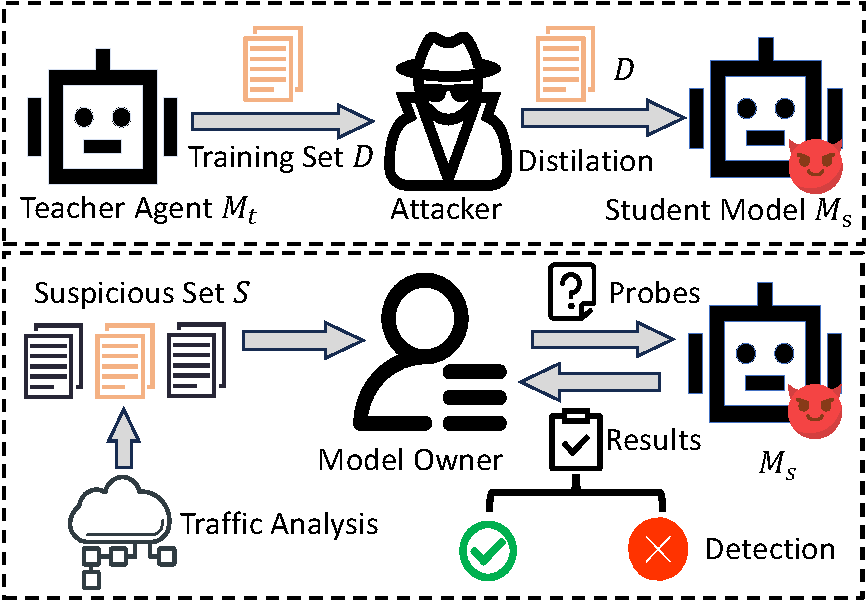
\includegraphics[width=0.95\columnwidth]{figure/seeting.pdf}
    \caption{Overview of the access and threat model. The attacker distills a student from trajectories, while the model owner identifies suspicious traffic and audits the student.}
    \label{fig:threat-model}
\end{figure}
We formulate a two-party threat model comprising a model owner and an attacker as shown in Figure~\ref{fig:threat-model}. The owner deploys a teacher model $\mathcal{M}_t$, while the attacker aims to distill a student model $\mathcal{M}_s$ using a training dataset $\mathcal{D}$ collected from the teacher model.

\partitle{Model Owner} The owner deploys and fully controls a teacher model $\mathcal{M}_t$ (e.g., Codex~\cite{singh2025openai}) as a service. To protect the model, the owner embeds watermarks into the output trajectories in real time. Since data scraping has specific patterns, the owner monitors server-side features~\cite{huh2025preventing, chiang2024chatbot, liu2026embarrassingly}. Any interactions showing such signs are recorded to build a suspicious trajectory set $\mathcal{S}$. To avoid missing potential distillation traces, the owner conservatively records all suspicious traces into $\mathcal{S}$ and the owner cannot determine which traces in $\mathcal{S}$ were actually used for distillation. When testing the deployed student model $\mathcal{M}_s$, the owner only has black box access and can fully control the API inputs to verify the watermark.


\partitle{Attacker}
To bypass the high training costs, the attacker aims to clone the capabilities of the teacher $\mathcal{M}_t$. Operating under strict black-box access, the attacker systematically queries the teacher model $\mathcal{M}_t$ to harvest complete multi-step interaction trajectories and this large-scale automated querying leaves identifiable server-side traffic patterns that can be captured by the model owner. The attacker may then preprocess these collected trajectories through operations such as sanitization, rewriting, truncation, or mixing with other data, forming the final distillation dataset $\mathcal{D}$. Finally, the attacker uses $\mathcal{D}$ to distill the student model $\mathcal{M}_s$ and deploys it as a black-box API.


\section{Watermark Construction}

\subsection{Overview}

During distillation, the distilled students and their teachers share similar interaction trajectories~\cite{yang2026agents, lyu2025correction, gudibande2023false}. Based on this property, we proposed a watermark scheme \name{} as illustrated in Figure~\ref{fig:overview}. Firstly, the owner embeds the watermark by dynamically inserting auxiliary(aux) behaviors into the teacher's trajectories and privately saves evidence. Once suspicious traffic is identified, the corresponding records are extracted to form an evidence pool in Section~\ref{sec:watermark_embedding}. Next, the owner uses this evidence to construct paired real and fake probes, applying statistical tests to verify if the suspect model reproduces the watermark in Section~\ref{Detection}. Finally, trace-level attribution in Section~\ref{subsec:trace_level} to evaluate which suspicious trajectories are most likely to have been used in the attacker's training set.

\begin{figure}[!t]
\centering
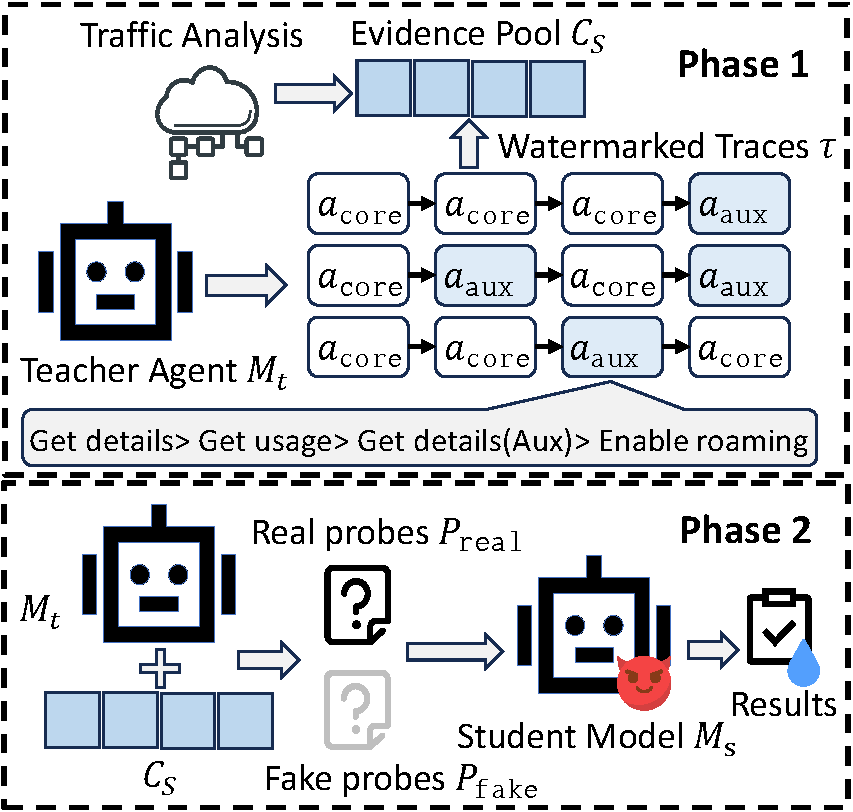
\includegraphics[width=0.95\columnwidth]{figure/overview.pdf}
\caption{Overview of \name{}. \textbf{Phase 1:} the owner embeds the watermark by inserting aux behaviors; \textbf{Phase 2:} the owner retrieves the private evidence to construct paired real and fake probes and verify a suspect student model. \textcolor[HTML]{BDD7EE}{\rule{0.85em}{0.85em}} denotes watermarked thing.}
\label{fig:overview}
\end{figure}

\subsection{Watermark Embedding Algorithm}

\label{sec:watermark_embedding}
Unlike previous watermarking methods that directly change the generated text or the teacher model's actions~\cite{wang2026protecting,an2026sequential}, \name{} embeds watermarks by adding extra, non-essential auxiliary actions into the agent's trajectory. By doing this, \name{} keeps the teacher model's performance high while creating strong evidence for later tracing. Also, to stay hidden, the added aux actions look and act exactly like normal tool calls: they use valid tools and bind strictly to normal parameter values derived from the interaction history. Based on the threat model described in Section \ref{sec:preliminaries}, the owner can subsequently identify suspicious traces from the API traffic and export their privately saved watermark evidence for later verification. The entire embedding process consists of three main stages shown in Figure\ref{fig:watermark_embedding_protocol}: safe tool classification, dynamic scheduling and candidate generation, and private evidence retention.

\partitle{Safe tool classification} To ensure aux actions will not change the environment state, \name{} applies a conservative safety policy to the tool schema $\mathcal{F}$ of trace $\tau$. Since LLM usually cooperating with agent system operates as an agent-as-a-service~\cite{li2026aidev}, this safety policy is performed in advance and cached to avoid real-time latency. An offline safety model $\mathcal{M}_{\mathtt{safe}}$ evaluates the tool schema $\mathcal{F}$ and maps each tool $f \in \mathcal{F}$ to a safety label as shown in Eq.\ref{equ:safeclassfier}:
\begin{equation}
\mathcal{M}_{\mathtt{safe}}(f)=\begin{cases}\mathtt{safe},&\text{if }f\text{ is read-only,}\\\mathtt{unsafe},&\text{otherwise.}\end{cases}
\label{equ:safeclassfier}
\end{equation}
The system exclusively permits tools from the valid subset $\mathcal{F}_{\mathtt{safe}}=\{f \in \mathcal{F} \mid \mathcal{M}_{\mathtt{safe}}(f)=\mathtt{safe}\}$, categorically rejecting any action that changes the environment state or influences the task process.

\partitle{Dynamic scheduling} Having established the safe tool subset $\mathcal{F}_{\mathtt{safe}}$, the system must determine when to invoke these aux action during the interaction as the watermarking. To make watermark positions unpredictable, \name{} dynamically evaluates whether to inject an aux action at step $t$ immediately after the core action $a_{\mathtt{core}}^{t-1}$ finishes. If skipped, the system waits and checks again after the next core action. For each trajectory $\tau$ named as $\mathtt{id}_\tau$ of an account $a$, the system keeps a release probability $p_t$ and a remaining budget $b_t$ at step $t$. Immediately after the core action $a_{\mathtt{core}}^{t-1}$ finishes, the system uses a cryptographic hash function $\mathtt{Hash}(\cdot) \to [0,1)$~\cite{preneel1994cryptographic} parameterized by the owner's secret key $k$ to compute a uniformly distributed random value $u_t$, as defined in Eq.~\ref{equ:hash}:
\begin{equation}
    \label{equ:hash}
u_t = \operatorname{\mathtt{Hash}}(k \mathbin\Vert a \mathbin\Vert \mathtt{id}_\tau \mathbin\Vert t) \in [0, 1).
\end{equation}
The system tries to add an aux action when $b_t>0$ and $u_t<p_t$. Depending on whether the auxiliary action is successfully inserted or the turn is skipped (due to generation failure or unmet conditions), the system updates the probability and budget for the next turn as follows:
\begin{equation}
\label{equ:pb_update}
(p_{t+1},b_{t+1})=
\left\{
\begin{array}{@{}l@{\;}l@{}}
(p_0,b_t-1), & \text{inserted},\\
(\min\{p_t+\Delta p,p_{\mathtt{max}}\},b_t),
& \text{otherwise}.
\end{array}
\right.
\end{equation}
\partitle{Aux action embedding} If the dynamic scheduling condition is met, \name{} proceeds to generate and select the optimal aux action. To obtain high quality insertions, the system queries $\mathcal{M}_t$ to propose up to $K$ candidates. Each candidate $j$ is formulated as a tuple of a thought and an action: $(t_{\mathtt{aux}}^j, a_{\mathtt{aux}}^j)$, where the action $a_{\mathtt{aux}}^j$ consists of a tool $f_{\mathtt{aux}}^j$ and its arguments $p_{\mathtt{aux}}^j$. To ensure that the injected action perfectly blends into the trajectory, \name{} enforces a validation mechanism. First, the chosen tool must belong to the safe subset $\mathcal{F}_{\mathtt{safe}}$. Second, to prevent model hallucinations and ensure contextual rationality, the arguments $p_{\mathtt{aux}}^j$ must be extracted from the context (such as the core action's observation or history). Consequently, \name{} categorically discards any candidate that uses an unapproved tool or hallucinates untraceable arguments.

For each candidate $j$ that passes the validation, \name{} employs a scoring model $\mathcal{M}_q$ to evaluate it across three dimensions: naturalness, logical consistency, and distillability. Specifically, $\mathcal{M}_q$ assigns a relevance score $s_{\mathtt{rel}}^j$ to ensure the injected action aligns naturally with the task. Additionally, a reliability score $s_{\mathtt{relb}}^j$ ensures the high quality of the thought. Crucially, to foster a stable behavioral habit that the student model can easily absorb during distillation, the system calculates a repeatability score $s_{\mathtt{rep}}^j$. This score is directly determined by $n_j$, which represents the number of times the candidate's specific tool pairing $(f_{\mathtt{core}}, f_{\mathtt{aux}}^j)$ has been successfully injected in the account's history. The final score $S_j$ for candidate $j$ is computed as a weighted sum:
\begin{equation}
    S_j = \alpha \cdot s_{\mathtt{rel}}^j + \beta \cdot s_{\mathtt{relb}}^j + \gamma \cdot s_{\mathtt{rep}}^j.
    \label{equ:score}
\end{equation}
where $\alpha$, $\beta$, $\gamma$, and the step-function mapping from repeat count $n_j$ to $s_{\mathtt{rep}}^j$ are detailed in Appendix~\ref{sec:experimental-details}. The system selects the candidate with the highest score as the best aux action $(t_{\mathtt{aux}}^{\mathtt{best}}, a_{\mathtt{aux}}^{\mathtt{best}})$, then injects this aux action, establishing a natural sequence:
\begin{equation}
    (
    t_{\mathtt{core}}^{t-1},
    a_{\mathtt{core}}^{t-1},
    o_{\mathtt{core}}^{t-1}
    )
    \;\rightarrow\;
    (
    t_{\mathtt{aux}}^{\mathtt{best}},
    a_{\mathtt{aux}}^{\mathtt{best}},
    o_{\mathtt{aux}}^{\mathtt{best}}
    ).
\end{equation}
Based on the generation result, the system updates its states. A successful generation applies the success update (Eq.~\ref{equ:pb_update}) and increases the repeat count $n_{\mathtt{best}}$ for this tool pairing. If the generation fails, the system skips the insertion, applies the failure update, moves to generate core action and waits for next chance. For future auditing, every successful insertion creates a private evidence card $c_t$. To securely record the exact context and execution details, this card stores the historical context $h$, the preceding core action and observation, and the injected auxiliary tool parameters. It is saved as a tuple and added to the trajectory's evidence set $\mathcal{C}_\tau = \mathcal{C}_\tau \cup \{c_t\}$:
\begin{equation}
    c_t = (h, t_{\mathtt{core}}^{t-1}, a_{\mathtt{core}}^{t-1}, o_{\mathtt{core}}^{t-1}, f_{\mathtt{aux}}^{\mathtt{best}}, p_{\mathtt{aux}}^{\mathtt{best}}).
    \label{equ:evidence}
\end{equation}
As mentioned in our threat model, the model owner uses signals like querying styles, IPs, and traffic patterns to identify a suspicious set $\mathcal{S}$~\cite{chiang2024chatbot, liu2026embarrassingly}. The owner then collects the evidence from these flagged traces to form a global verification pool $\mathcal{C}_{\mathcal{S}} = \bigcup_{\tau \in \mathcal{S}} \mathcal{C}_\tau$.


\subsection{Watermark Verification}

\label{Detection}
While the embedding phase injects an aux action into the teacher's trajectory, the tracing phase verifies if a suspect model $M_s$ has learned this specific behavior pattern. To achieve this, \name{} uses paired probes built from the combined evidence pool $\mathcal{C}_{\mathcal{S}}$ for verification as shown in Figure~\ref{fig:watermark_detection_protocol}.



\partitle{Paired probe construction} To verify watermark retention, \name{} constructs paired probes for the combined evidence pool $\mathcal{C}_{\mathcal{S}}$. A probe is formally defined as a prompt-target tuple: given a history and a core action as the prompt, the suspect model $\mathcal{M}_s$ is expected to output a specific aux action. Specifically, based on each evidence card, we derive two types of probes: real probes and  fake probes. This paired design ensures that the model $\mathcal{M}_s$ has genuinely memorized the specific watermarked trace, rather than unconditionally outputting the target action.

For the real side construction of each card $c_i \in \mathcal{C}_S$, the system first locates the nearest core action. To ensure that the suspect model $M_s$ has learned the expected behavior, \name{} creates up to $N$ parameterized variants for this real side by modifying one argument of the original core action, the system prompts the teacher model $\mathcal{M}_t$ to synchronously generate a logically consistent core triplet $(t_{\mathtt{core}}^j, a_{\mathtt{core}}^j, o_{\mathtt{core}}^j)$ alongside the new downstream target aux arguments $p_{\mathtt{aux}}^j$. This process directly generates a set of real side probes $p_{\mathtt{real}}^i$ for the specific card $c_i$ as shown in Eq.\ref{equ:probe real}:
    
\begin{equation}
    \label{equ:probe real}
p_{\mathtt{real}}^i = \left\{ (h, t_{\mathtt{core}}^j, a_{\mathtt{core}}^j, o_{\mathtt{core}}^j),\ (f_{\mathtt{aux}}, p_{\mathtt{aux}}^j)  \right\}_{j=1}^{N_i}.
\end{equation}
$h$ is the historical context, and $f_{\mathtt{aux}}$ is the targeted aux tool. Finally, the system aggregates the real-side probes from all cards to form the global real probe set $\mathcal{P}_{\mathtt{real}} = \bigcup_{c_i \in \mathcal{C}_S} p_{\mathtt{real}}^i$.

To better contrast with the real probes $\mathcal{P}_{\mathtt{real}}$, obtain more definitive statistical results, \name{} constructs a set of fake probes based on the $\mathcal{P}_{\mathtt{real}}$. This verifies whether the aux action stems from memorization rather than natural context or random chance.For this fake side. However, it prompts the teacher model $\mathcal{M}_t$ to replace the core action with a semantically similar fake core behavior $(\hat{t}_{\mathtt{core}}^j, \hat{a}_{\mathtt{core}}^j,\hat{o}_{\mathtt{core}}^j)$ that achieves the identical goal. This process generates the fake probe set $p_{\mathtt{fake}}^i$ for card $c_i$, directly matching the variants in $p_{\mathtt{real}}^i$ as shown in Eq.\ref{probe fake}:
    
\begin{equation}
    \label{probe fake}
p_{\mathtt{fake}}^i = \left\{  (h, \hat{t}_{\mathtt{core}}^j, \hat{a}_{\mathtt{core}}^j, \hat{o}_{\mathtt{core}}^j),\ (f_{\mathtt{aux}}, p_{\mathtt{aux}}^j)  \right\}_{j=1}^{N_i}.
\end{equation}
Thus, the strict difference between the paired probes lies only in the core action. Similar to the real side, the fake probe set is defined as $\mathcal{P}_{\mathtt{fake}} = \bigcup_{c_i \in \mathcal{C}_S} p_{\mathtt{fake}}^i$.

\partitle{Card-level statistical test} After generating the paired probes, \name{} evaluates the suspect model $M_s$ using $(\mathcal{P}_{\mathtt{real}}, \mathcal{P}_{\mathtt{fake}})$ and performs a card-level statistical test which is discussed in Appendix~\ref{sec:statistical-test-discussion}. For the $j$-th probe pair of card $c_i$, the expected aux action is $f_{\mathtt{aux}}$ and arguments $p_{\mathtt{aux}}^j$. Let $(f_{\mathtt{out}}, p_{\mathtt{out}})$ be the tool call parsed from the output of $M_s$. For both real and fake sides, \name{} computes the toolhit indicator $t_{i,j}$ and the fullhit indicator $h_{i,j} \in \{0, 1\}$:

\begin{equation}
t_{i,j} = \operatorname{\mathtt{Mat}}(f_{\mathtt{out}}, f_{\mathtt{aux}}),\quad h_{i,j} = t_{i,j} \cdot \operatorname{\mathtt{Mat}}(p_{\mathtt{out}}, p_{\mathtt{aux}}^j).
\label{eq:probe-score}
\end{equation}
where the function $\operatorname{\mathtt{Mat}}(\cdot, \cdot) \to \{0, 1\}$ evaluates to $1$ if and only if there is exact structural and value equivalence between its two arguments, and $0$ otherwise. Because the $N_i$ paired variants derived from the same card $c_i$ share an identical core-to-aux dependency, they are not independent samples. Therefore, \name{} aggregates the scores at the card level to calculate the real-side hit rate $R_i^{\mathtt{real}}$, the fake-side hit rate $R_i^{\mathtt{fake}}$, and their difference $\Delta_i$ for each card $c_i$ as shown in Eq.\ref{eq:probe-rate}:
\begin{equation}
\begin{gathered}
R_i^{\mathtt{real}}
= \frac{1}{N_i}\sum_{j=1}^{N_i}h_{i,j}^{\mathtt{real}},
\quad
R_i^{\mathtt{fake}}
= \frac{1}{N_i}\sum_{j=1}^{N_i}h_{i,j}^{\mathtt{fake}},\\
\Delta_i
= R_i^{\mathtt{real}}-R_i^{\mathtt{fake}}.
\end{gathered}
\label{eq:probe-rate}
\end{equation}
To evaluate the verification, we establish the null hypothesis $H_0$ and the alternative hypothesis $H_1$. $H_0$ posits that the suspect model $\mathcal{M}_s$ has not learned the watermarked habit; any correct action is due to general context or innate biases. Conversely, $H_1$ asserts that $\mathcal{M}_s$ has memorized the watermark, making it significantly more likely to output the target action on real probes. Based on the performance difference $\Delta_i$ for each card $c_i$, we classify the outcomes into a real win ($\Delta_i > 0$), a fake win ($\Delta_i < 0$), or a tie ($\Delta_i = 0$). Excluding ties, let $w$ and $\ell$ be the numbers of real and fake wins across $\mathcal{C}_{\mathcal{S}}$. The $p$-value is computed using a one-sided exact sign-test~\cite{hollander2013nonparametric}:

\begin{equation}
    p\mathtt{-value} = \sum_{k=w}^{w+\ell}\binom{w+\ell}{k}2^{-(w+\ell)}.
\end{equation}
where $p\mathtt{-value} = 1$ if $w+\ell=0$. To reject $H_0$ and declare a successful verification, \name{} requires dual criteria: the statistical significance must be $p\mathtt{-value} < p$, and the averaged real fullhit rate must exceed the fake rate by a predefined margin $r$ (i.e., $\frac{1}{|\mathcal{C}_{\mathcal{S}}|} \sum \Delta_i \geq r$). This margin absorbs unpredictable fluctuations caused by context rewriting in the fake probes and guards against false positives. Appendix~\ref{sec:experimental-details} specifies the hyperparameters $p$, $r$, and $N$.


\subsection{Trace-Level Attribution} \label{subsec:trace_level}

While the verification protocol in Section~\ref{Detection} determines whether a suspect model $\mathcal{M}_s$ has distilled from $\mathcal{M}_t$, it cannot pinpoint which traces within $\mathcal{S}$ were utilized. For exact attribution, \name{} introduces a trace-level attribution. For each evaluated trace $\tau$, the system computes four rates to capture both exact and partial matches: the strict full-hit rates $R_\tau^{\mathtt{real}}$ and $R_\tau^{\mathtt{fake}}$, and the toolhit-only rates $T_\tau^{\mathtt{real}}$ and $T_\tau^{\mathtt{fake}}$ (where $t_{i,j}=1 \land h_{i,j}=0$). To ensure fair comparison across traces, \name{} normalizes each rate into an average-rank quantile $Q(\cdot) \in (0, 1)$:

\begin{equation}
    Q(x_\tau) = \frac{\operatorname{\mathtt{rank}}_{\mathtt{avg}}(x_\tau)}{|\mathcal{S}| + 1}.
\end{equation}
The attribution logic is designed as follows: $Q(R_\tau^{\mathtt{real}})$ acts as the primary positive signal for trace memorization. Conversely, if the model outputs the target aux action even on the fake probes, it implies innate biases rather than specific watermark retention. Thus, $Q(R_\tau^{\mathtt{fake}})$ serves as a penalty term. Furthermore, the toolhit-only terms address partial memorization, providing supplementary evidence to calibrate the final score. Consequently, \name{} ranks these traces using a score $S_\tau$:
    
\begin{equation}
\!S_\tau\!=\!Q(R_\tau^{\mathtt{real}})
 \!-\!\alpha'Q(R_\tau^{\mathtt{fake}})
 \!+\!\beta'Q(T_\tau^{\mathtt{real}})
 \!-\!\gamma'Q(T_\tau^{\mathtt{fake}}).
\label{eq:trace-score}
\end{equation}
where the empirical weighting parameters $\alpha'$, $\beta'$, and $\gamma'$ are detailed in Appendix~\ref{sec:experimental-details}. Finally, the system identifies the top-$K$ traces with the highest $S_\tau$ most likely included in the training set $\mathcal{D}$.


\section{Experiments}
    
\label{sec:experiments}
\subsection{Experimental Setup}
    
We evaluate \name{} in agent distillation. We supervise thoughts and actions from the trajectories and fine-tune the student models using LoRA. The specific training configurations are rank $32$, learning rate $2\times10^{-4}$, and $\alpha = 64$. Prior traffic-analysis systems have reported identification precision above $70\%$~\cite{chiang2024chatbot, liu2026embarrassingly}. We therefore adopt a more conservative $50\%$ precision setting to avoid missing potential distillation traces, with $|\mathcal{S}|=100$ suspicious trajectories and $|\mathcal{D}_c|=50$ trajectories used for distillation. Appendix~\ref{sec:experimental-details} provides the remaining experimental details, including hyperparameter selection and baselines. Our experiments assess watermark effectiveness, harmlessness, robustness against adversarial processing.

\partitle{Datasets and Models} Our evaluation spans three datasets: BFCL~\cite{patil2025berkeley}, SWE-bench~\cite{jimenez2024swe}, and Telecom (a service-tool domain from the Tau2 benchmark\footnote{\url{https://github.com/sierra-research/tau2-bench}}). GPT-OSS-120B~\cite{agarwal2025gpt} and Kimi-K2.5~\cite{team2026kimi} serve as teacher agents ($\mathcal{M}_t$), with Qwen3-8B acting as both the candidate scorer ($\mathcal{M}_q$) and safety model ($\mathcal{M}_{\mathtt{safe}}$). For distillation, we fine-tune four student models ($\mathcal{M}_s$): Mistral-Small-3.1-24B~\cite{liu2026ministral}, Qwen3-14B~\cite{yang2025qwen3}, Qwen3-32B~\cite{yang2025qwen3}, and GLM-4.7-Flash~\cite{glm2024chatglm}.

\partitle{Evaluation metrics} For detection, we report strict fullhit rates $(R_\tau^{\mathtt{real}},R_\tau^{\mathtt{fake}})$ on real and fake probes, alongside the one-sided $p$-value. A successful detection requires $p<0.05$ and a real-fake mean fullhit gap $\ge 0.05$. For trace-level attribution, we measure $\operatorname{\mathtt{Precision}}@K$ of top-$K$ trajectories belonging to the distillation subset $\mathcal{D}_c$. For harmlessness, we compare task accuracy ($\mathtt{Acc}$) and mean interaction steps ($L$) between control and watermarked agents.

\subsection{Effectiveness}

\label{sec:detection-effectiveness}

\begin{table*}[!t]
\centering
\setlength{\tabcolsep}{3.5pt}
\caption{True-positive results. Cards is the number of cards; hit-rate cells report hits / probes (rate). $w/\ell$ gives card-level real / fake wins. The `Sig' column indicates statistical significance: {\color{green}$\checkmark$} denotes $p < 0.05$, indicating a statistically significant change, whereas {\color{red}$\times$} denotes $p \ge 0.05$.}

\label{tab:true-positive}
\scriptsize
\begin{tabular}{l l c l | c c c c c}
\noalign{\hrule height 1.5pt}
\multirow{2}{*}{\textbf{Teacher Agent$\mathcal{M}_t$}} & \multirow{2}{*}{\textbf{Dataset}} & \multirow{2}{*}{\textbf{Cards}} & \multirow{2}{*}{\textbf{Student Model $\mathcal{M}_s$}} & \multicolumn{5}{c}{\textbf{Detection Results}} \\
\cline{5-9}
& & & & \textbf{$R^{\mathtt{real}}$ (\%)} & \textbf{$R^{\mathtt{fake}}$ (\%)} & \textbf{$w/\ell$} & \textbf{$p$-value} & \textbf{Sig.} \\
\hline
\multirow{4}{*}{GPT-OSS-120B} & \multirow{4}{*}{BFCL} & \multirow{4}{*}{118} & Mistral-24B & \tableRate{93}{182}{51.1} & \tableRate{59}{182}{32.4} & 25 / 1 & \tablePval{4.0}{-7} & {\color{green}\checkmark} \\
& & & GLM-4.7-Flash & \tableRate{108}{182}{59.3} & \tableRate{80}{182}{44.0} & 19 / 1 & \tablePval{2.0}{-5} & {\color{green}\checkmark} \\
& & & Qwen3-14B & \tableRate{44}{182}{24.2} & \tableRate{28}{182}{15.4} & 20 / 4 & \tablePval{7.7}{-4} & {\color{green}\checkmark} \\
& & & Qwen3-32B & \tableRate{89}{182}{48.9} & \tableRate{58}{182}{31.9} & 30 / 9 & \tablePval{5.3}{-4} & {\color{green}\checkmark} \\
\hline
\multirow{4}{*}{Kimi-K2.5} & \multirow{4}{*}{BFCL} & \multirow{4}{*}{145} & Mistral-24B & \tableRate{175}{379}{46.2} & \tableRate{105}{379}{27.7} & 45 / 10 & \tablePval{1.0}{-6} & {\color{green}\checkmark} \\
& & & GLM-4.7-Flash & \tableRate{155}{379}{40.9} & \tableRate{69}{379}{18.2} & 47 / 4 & \tablePval{1.2}{-10} & {\color{green}\checkmark} \\
& & & Qwen3-14B & \tableRate{102}{379}{26.9} & \tableRate{26}{379}{6.9} & 46 / 4 & \tablePval{2.2}{-10} & {\color{green}\checkmark} \\
& & & Qwen3-32B & \tableRate{82}{379}{21.6} & \tableRate{18}{379}{4.7} & 39 / 5 & \tablePval{7.0}{-8} & {\color{green}\checkmark} \\
\noalign{\hrule height 1.5pt}
\end{tabular}
\end{table*}


In this section, all student models are trained on the original  dataset $\mathcal{D}_c$. We test our scheme on distilled and clean models via separate true positive and false positive experiments. We also evaluate the performance of existing agent watermark baselines under the matched setting. Furthermore, we evaluate \name{}'s trace-level attribution using $\operatorname{\mathtt{Precision}}@K$ in Appendix~\ref{sec:supplementary-effectiveness}. Finally, we measure how identification accuracy affects statistical significance in Appendix~\ref{sec:supplementary-effectiveness}.



\partitle{True positives} We first evaluate whether \name{} can successfully identify student models distilled from watermarked trajectories. Our experiments cover all combinations of 3 datasets (SWE and Telecom are in Appendix~\ref{sec:supplementary-effectiveness}), 2 teacher agents, and 4 student models. In each setting, we compare the hit rates between the real side and the fake side and calculate the $p$-value. The results in the Table~\ref{tab:true-positive} and~\ref{tab:appendix-true-positive} show that \name{} successfully achieves detection in all settings. These results show that \name{} can extract watermark from student models of different architectures.


\partitle{False positives} We evaluate whether \name{} causes false positives on clean models that have not seen watermarked trajectories. As shown in Table~\ref{tab:false-positive} and Table~\ref{tab:appendix-false-positive} in Appendix~\ref{sec:supplementary-effectiveness}, in addition to the four undistilled student models, we also select four base models (DeepSeek-V4-Flash \cite{xu2026deepseek}, MiniMax-M2.5 \cite{chen2026minimax}, Qwen3.5-Flash \cite{yang2025qwen3}, and MiMo-V2.5 \cite{xiao2026mimo}) and build a total of 48 controlled false-positive evaluation settings. The results show that \name{} achieves zero false positives across all 48 settings.

\begin{table*}[!t]
\caption{False-positive results. The `Sig' column indicates statistical significance: {\color{green}$\checkmark$} denotes $p < 0.05$, indicating a statistically significant change, whereas {\color{red}$\times$} denotes $p \ge 0.05$.}
\label{tab:false-positive}
\centering
\setlength{\tabcolsep}{5.3pt}
\scriptsize
\begin{tabular}{l l c l | c c c c c}
\noalign{\hrule height 1.5pt}
\multirow{2}{*}{\textbf{Teacher Agent$\mathcal{M}_t$}} & \multirow{2}{*}{\textbf{Dataset}} & \multirow{2}{*}{\textbf{Cards}} & \multirow{2}{*}{\textbf{Clean Model $\mathcal{M}_c$}} & \multicolumn{5}{c}{\textbf{Detection Results}} \\
\cline{5-9}
& & & & \textbf{$R^{\mathtt{real}}$ (\%)} & \textbf{$R^{\mathtt{fake}}$ (\%)} & \textbf{$w/\ell$} & \textbf{$p$-value} & \textbf{Sig.} \\
\hline
\multirow{8}{*}{GPT-OSS-120B} & \multirow{8}{*}{BFCL} & \multirow{8}{*}{118} & DeepSeek-V4-Flash & \tableRate{10}{182}{5.5} & \tableRate{11}{182}{6.0} & 2 / 3 & \tablePval{8.1}{-1} & {\color{red}$\times$} \\
& & & MiniMax-M2.5 & \tableRate{9}{182}{4.9} & \tableRate{10}{182}{5.5} & 2 / 3 & \tablePval{8.1}{-1} & {\color{red}$\times$} \\
& & & Mistral-24B & \tableRate{9}{182}{4.9} & \tableRate{7}{182}{3.8} & 3 / 2 & \tablePval{5.0}{-1} & {\color{red}$\times$} \\
& & & Qwen3-14B & \tableRate{7}{182}{3.8} & \tableRate{6}{182}{3.3} & 2 / 1 & \tablePval{5.0}{-1} & {\color{red}$\times$} \\
& & & Qwen3-32B & \tableRate{4}{182}{2.2} & \tableRate{4}{182}{2.2} & 2 / 2 & \tablePval{6.9}{-1} & {\color{red}$\times$} \\
& & & Qwen3.5-Flash & \tableRate{8}{182}{4.4} & \tableRate{8}{182}{4.4} & 2 / 1 & \tablePval{5.0}{-1} & {\color{red}$\times$} \\
& & & MiMo-V2.5 & \tableRate{10}{182}{5.5} & \tableRate{11}{182}{6.0} & 2 / 2 & \tablePval{6.9}{-1} & {\color{red}$\times$} \\
& & & GLM-4.7-Flash & \tableRate{5}{182}{2.7} & \tableRate{1}{182}{0.5} & 4 / 0 & \tablePval{6.2}{-2} & {\color{red}$\times$} \\
\hline
\multirow{8}{*}{Kimi-K2.5} & \multirow{8}{*}{BFCL} & \multirow{8}{*}{145} & DeepSeek-V4-Flash & \tableRate{10}{379}{2.6} & \tableRate{9}{379}{2.4} & 5 / 4 & \tablePval{5.0}{-1} & {\color{red}$\times$} \\
& & & MiniMax-M2.5 & \tableRate{6}{379}{1.6} & \tableRate{3}{379}{0.8} & 4 / 2 & \tablePval{3.4}{-1} & {\color{red}$\times$} \\
& & & Mistral-24B & \tableRate{1}{379}{0.3} & \tableRate{3}{379}{0.8} & 1 / 2 & \tablePval{8.8}{-1} & {\color{red}$\times$} \\
& & & Qwen3-14B & \tableRate{1}{379}{0.3} & \tableRate{0}{379}{0.0} & 1 / 0 & \tablePval{5.0}{-1} & {\color{red}$\times$} \\
& & & Qwen3-32B & \tableRate{1}{379}{0.3} & \tableRate{0}{379}{0.0} & 1 / 0 & \tablePval{5.0}{-1} & {\color{red}$\times$} \\
& & & Qwen3.5-Flash & \tableRate{0}{379}{0.0} & \tableRate{0}{379}{0.0} & 0 / 0 & \tablePval{1.0}{0} & {\color{red}$\times$} \\
& & & MiMo-V2.5 & \tableRate{6}{379}{1.6} & \tableRate{6}{379}{1.6} & 4 / 3 & \tablePval{5.0}{-1} & {\color{red}$\times$} \\
& & & GLM-4.7-Flash & \tableRate{2}{379}{0.5} & \tableRate{2}{379}{0.5} & 2 / 1 & \tablePval{5.0}{-1} & {\color{red}$\times$} \\
\noalign{\hrule height 1.5pt}
\end{tabular}
\end{table*}






\partitle{Baseline effectiveness} AgentWM and SeqWM show limited detectability under our tested distillation configurations. Section~\ref{sec:systematization-findings} discusses this finding; Appendix~\ref{sec:watermark-limitations} reports the per-model results and decision rules. Because the methods use different detection statistics, these results do not constitute a comparison at a common false-positive rate.

\subsection{Harmlessness}
\label{sec:harmlessness}

\partitle{Harmlessness} A reasonable watermark scheme should not noticeably affect the performance of the teacher agent. Therefore, we evaluate impact of \name{} on the teacher agent $\mathcal{M}_t$'s task utility and inference cost. For the four cohorts in BFCL and Telecom, we compare the unwatermarked agent $\mathcal{M}_\mathtt{tc}$ and the watermarked teacher agent $\mathcal{M}_t$ on 200 tasks. We measure the task accuracy difference $\Delta \mathtt{Acc} = \mathbb{E}[\mathtt{Acc}(\mathcal{M}_t) - \mathtt{Acc}(\mathcal{M}_\mathtt{tc})]$ and the expected interaction step difference $\Delta L = \mathbb{E}[L(\mathcal{M}_t) - L(\mathcal{M}_\mathtt{tc})]$. As summarized in Figure~\ref{fig:harmlessness}, embedding the watermark does not cause a drop in overall performance. The task accuracy difference $\Delta \mathtt{Acc}$ ranges only from $-3.0\%$ to $+3.0\%$, indicating that the accuracy loss is acceptable. Meanwhile, the increase in interaction cost is acceptable: the average step count increases from 20.49 to 21.09 steps, and $\Delta L$ ranges from $-1.38$ to $+2.04$ steps.

\begin{figure*}[!t]
\centering
\begin{subfigure}[t]{0.242\textwidth}
\centering
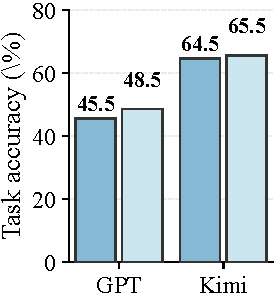
\includegraphics[width=0.82\linewidth]{figure/harmlessness_accuracy_bfcl.pdf}
\caption{BFCL: accuracy}
\end{subfigure}\hfill
\begin{subfigure}[t]{0.242\textwidth}
\centering
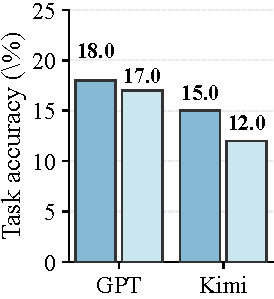
\includegraphics[width=0.82\linewidth]{figure/harmlessness_accuracy_telecom.pdf}
\caption{Telecom: accuracy}
\end{subfigure}\hfill
\begin{subfigure}[t]{0.242\textwidth}
\centering
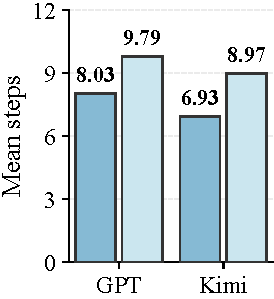
\includegraphics[width=0.82\linewidth]{figure/harmlessness_steps_bfcl.pdf}
\caption{BFCL: steps}
\end{subfigure}\hfill
\begin{subfigure}[t]{0.242\textwidth}
\centering
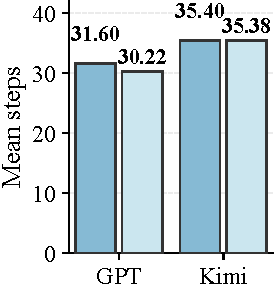
\includegraphics[width=0.82\linewidth]{figure/harmlessness_steps_telecom.pdf}
\caption{Telecom: steps}
\end{subfigure}
\caption{
Harmlessness results. In (a) and (b), the vertical axis reports accuracy; in (c) and (d), it reports the mean number of steps. Colors distinguish \textcolor[HTML]{86BAD4}{$\blacksquare$} unwatermarked and \textcolor[HTML]{CBE6EF}{$\blacksquare$} watermarked runs.
}

\label{fig:harmlessness}
\end{figure*}


\subsection{Robustness}
\label{sec:robustness}

To demonstrate the robustness of our watermark scheme, We evaluate \name{}'s robustness against four common pre-distillation data transformations. These operations include: data flooding, paraphrasing attack, adaptive attack, advanced data flooding and truncation (the last two are in Appendix~\ref{sec:supplementary-robustness}). We evaluate the robustness of Agentwm under data flooding in Appendix~\ref{sec:supplementary-robustness}. We use GPT-OSS-120B as the teacher agent.

\partitle{Data flooding} Before distillation, an attacker may mix the training set with standard clean data to improve distillation performance~\cite{ouyang2022training, mukherjee2023orca}, which will dilutes the watermark signals. To evaluate its impact on our watermark strength, we mix the original watermarked dataset $\mathcal{D}_c$ with clean standard answers. Specifically, in the D1, D5, and D10 settings, we incorporate $1\times$, $5\times$, and $10\times$ the amount of clean data relative to $\mathcal{D}_c$. We evaluate a total of 24 settings across 2 benchmarks (BFCL and SWE-bench), 3 dilution ratios, and 4 student models. As shown in Figure~\ref{fig:data-flooding-robustness}, \name{} successfully detects every setting. Even under the strongest $1{:}10$ dilution ratio, all 8 tested student models remain successfully detected.
\begin{figure*}[!t]
\centering
\begin{subfigure}[t]{\robustnessPanelWidth}
\centering
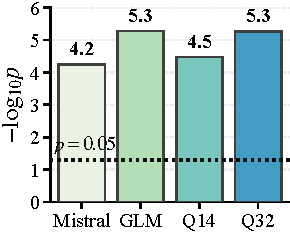
\includegraphics[width=0.72\linewidth]{figure/robustness_data_flooding_bfcl_d1.pdf}
\caption{BFCL: D1}
\end{subfigure}\hfill
\begin{subfigure}[t]{\robustnessPanelWidth}
\centering
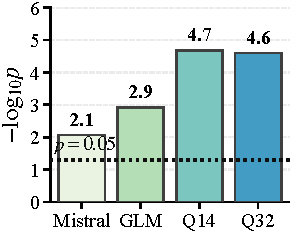
\includegraphics[width=0.72\linewidth]{figure/robustness_data_flooding_bfcl_d5.pdf}
\caption{BFCL: D5}
\end{subfigure}\hfill
\begin{subfigure}[t]{\robustnessPanelWidth}
\centering
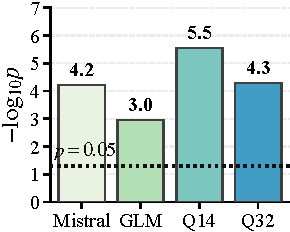
\includegraphics[width=0.72\linewidth]{figure/robustness_data_flooding_bfcl_d10.pdf}
\caption{BFCL: D10}
\end{subfigure}\par
\begin{subfigure}[t]{\robustnessPanelWidth}
\centering
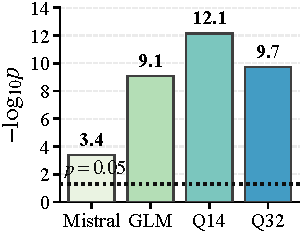
\includegraphics[width=0.72\linewidth]{figure/robustness_data_flooding_swe_bench_d1.pdf}
\caption{SWE-bench: D1}
\end{subfigure}\hfill
\begin{subfigure}[t]{\robustnessPanelWidth}
\centering
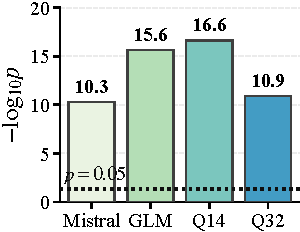
\includegraphics[width=0.72\linewidth]{figure/robustness_data_flooding_swe_bench_d5.pdf}
\caption{SWE-bench: D5}
\end{subfigure}\hfill
\begin{subfigure}[t]{\robustnessPanelWidth}
\centering
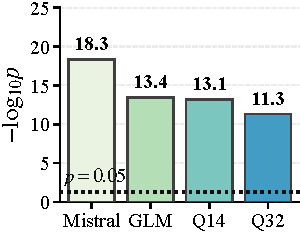
\includegraphics[width=0.72\linewidth]{figure/robustness_data_flooding_swe_bench_d10.pdf}
\caption{SWE-bench: D10}
\end{subfigure}

\caption{Data-flooding robustness. The vertical axis reports $-\log_{10}p$. In (a)--(f), \robustnessModelLegend. The \textcolor[HTML]{8C8C8C}{\hdashrule[0.5ex]{1.2em}{1.2pt}{1pt 1.5pt}} marks $p=0.05$.}

\label{fig:data-flooding-robustness}
\end{figure*}

\begin{table}[!t]
\centering
\caption{Paraphrasing attack robustness.}
\label{tab:semantic-rewriting-robustness}
\scriptsize
\setlength{\tabcolsep}{2pt}
\begin{tabular*}{\linewidth}{@{\extracolsep{\fill}}l l | c c@{}}
\noalign{\hrule height 1.5pt}
\textbf{Dataset} & \textbf{Student Model $\mathcal{M}_s$} & \textbf{$p$-value} & \textbf{Sig.} \\
\hline
\multirow{4}{*}{BFCL} & Mistral-24B & \tablePval{5.7}{-5} & {\color{green}\checkmark} \\
& GLM-4.7-Flash & \tablePval{1.4}{-4} & {\color{green}\checkmark} \\
& Qwen3-14B & \tablePval{3.3}{-3} & {\color{green}\checkmark} \\
& Qwen3-32B & \tablePval{9.8}{-5} & {\color{green}\checkmark} \\
\hline
\multirow{4}{*}{Telecom} & Mistral-24B & \tablePval{3.2}{-2} & {\color{green}\checkmark} \\
& GLM-4.7-Flash & \tablePval{1.4}{-5} & {\color{green}\checkmark} \\
& Qwen3-14B & \tablePval{3.5}{-3} & {\color{green}\checkmark} \\
& Qwen3-32B & \tablePval{4.1}{-3} & {\color{green}\checkmark} \\
\noalign{\hrule height 1.5pt}
\end{tabular*}
\end{table}
\partitle{Paraphrasing attack} An attacker may paraphrase the trajectories, aiming to alter semantic patterns and evade watermark detection while preserving the utility~\cite{krishna2023paraphrasing}. To evaluate the robustness against this rewriting attack, we use DeepSeek-V4-Flash to paraphrase the  $\mathcal{D}_c$. Subsequently, we train 4 student models on these rewritten datasets across the BFCL and Telecom and detect their watermark signals. As reported in Table~\ref{tab:semantic-rewriting-robustness}, \name{} successfully detects the watermark across all 8 settings showing our scheme's robustness under paraphrasing.

\begin{table}[!t]
\centering
\caption{Adaptive attack robustness.}
\label{tab:adaptive-attack}
\scriptsize
\setlength{\tabcolsep}{2pt}
\begin{tabular*}{\linewidth}{@{\extracolsep{\fill}}l l | c c@{}}
\noalign{\hrule height 1.5pt}
\textbf{Dataset} & \textbf{Student Model $\mathcal{M}_s$} & \textbf{$p$-value} & \textbf{Sig.} \\
\hline
\multirow{4}{*}{BFCL} & Mistral-24B & \tablePval{9.2}{-4} & {\color{green}\checkmark} \\
& GLM-4.7-Flash & \tablePval{1.4}{-4} & {\color{green}\checkmark} \\
& Qwen3-14B & \tablePval{9.6}{-3} & {\color{green}\checkmark} \\
& Qwen3-32B & \tablePval{4.1}{-4} & {\color{green}\checkmark} \\
\hline
\multirow{4}{*}{Telecom} & Mistral-24B & \tablePval{2.8}{-8} & {\color{green}\checkmark} \\
& GLM-4.7-Flash & \tablePval{3.7}{-3} & {\color{green}\checkmark} \\
& Qwen3-14B & \tablePval{1.0}{-11} & {\color{green}\checkmark} \\
& Qwen3-32B & \tablePval{5.5}{-12} & {\color{green}\checkmark} \\
\noalign{\hrule height 1.5pt}
\end{tabular*}
\end{table}
\partitle{Adaptive attack} In this section, we consider a stronger attacker who knows that our watermark relies on auxiliary behaviors. To avoid detection, the attacker uses DeepSeek-V4-Flash to clean the collected data by finding and removing suspected auxiliary action while keeping the trajectories useful. Next, we fine-tune student models on this cleaned data and test them on BFCL and Telecom. As shown in Table~\ref{tab:adaptive-attack}, even with this removal, \name{} successfully detects all student models (with the minimal $p$-value of $9.6\times10^{-3}$). This shows that our watermark is highly robust, even when an attacker actively tries to move the signals.



\section{Conclusion}
\label{sec:conclusion}

We present \name{}, a behavioral watermarking framework to track the unauthorized distillation of LLM agents. \name{} inserts useful extra tool calls after normal core actions. To verify if the watermark is copied, it uses paired real and fake probes along with a card-level sign test. This design supports both model-level detection and trace-level tracking.In experiments across three benchmarks, two teacher models, and four student architectures, \name{} successfully detects all 24 distilled students with zero false positives on 48 clean models. It also remains highly effective under data flooding, rewriting, truncation, and adaptive cleaning attacks. Future work will extend this evaluation to more teacher models, cleaning tools, and training methods.







\bibliographystyle{IEEEtranN}
\bibliography{09_reference}

\appendices

% TODO: Add proofs, implementation details, supplementary experiments, and
% complete prompts or protocols here.

\section{Related Work}

\subsection{Model Distillation}
Knowledge distillation is originally proposed as to transfer the capicity of a teacher model to a student model \cite{hinton2015distilling}. With rapid development of LLM, fine-tuning on teacher-generated data has become an increasingly important form of distillation, allowing student models to acquire advanced capabilities directly from the teacher's responses \cite{hsieh2023distilling, mukherjee2023orca}. This paradigm has also been extended to agent systems \cite{kang2026distilling, liu2026structured, luo2026agentark}. Agent Distillation \cite{kang2026distilling} proposed an agent distillation method that enables student model to learn both tool-use behaviors and reasoning capabilities. AgentArk \cite{luo2026agentark} introduced a method that distills multi-agent dynamics into the weights of a single model. Agent trajectories record not only generated text but also tool use and multi-step decisions, making them valuable supervision for distillation. As these trajectories can be used to cheaply transfer the capabilities of teacher agents, unauthorized distillation poses a growing threat to model copyright and calls for effective detection and tracing mechanisms.


\subsection{Model Watermarking}



\partitle{Content watermarking}
Recent studies have proposed a series of content watermarking methods to identify whether a given output is generated by a specific model. Early methods mainly embed statistical signals during token generation, such as the red-green list mechanism \cite{kirchenbauer2023watermark}. Later studies further improve the robustness and generation quality of watermarks by using semantic information \cite{liu2024semantic, huo2026pmark, huo2026samark,hou2024semstamp}. However, with the development of LLM agents, traditional content watermarks are difficult to directly apply to agent settings. These methods usually embed watermark signals by changing token choices or semantic expressions in free-form text, while the key outputs of agents are often tool calls with strict format requirements. Directly modifying these outputs may break the tool calls and affect correct execution. Therefore, recent studies have started to move watermarks from generated content to agent trajectories and behavior patterns \cite{huang2025agent, an2026sequential, zhang2026memmark}.


\partitle{Model watermarking against distillation}
Several watermarking methods have been proposed to protect models against unauthorized distillation. Methods such as Lexical Watermark and CATER insert special word patterns into teacher outputs, so that student models trained on these outputs can inherit detectable features~\cite{he2022protecting, he2022cater, yang2026asking}. Recent work further targets LLM distillation by changing token generation or rewriting reasoning traces, either reducing the value of teacher outputs for distillation or leaving detectable signals in the student model~\cite{savani2026antidistillation, xu2026antidistillation, ma2026protecting}. However, these methods mainly work on text tokens or reasoning traces, and are difficult to directly apply to agents whose behavior is mainly represented by structured tool calls and multi-step interactions. Recent work has extended anti-distillation watermarking to agent trajectories~\cite{wang2026protecting}, but its main evaluation still focuses on settings where the teacher and student models use the same base model, and its robustness to data processing such as data mixing remains limited. Therefore, a more general and robust watermarking method is still needed for tracing agent distillation.




\section{Supplement of Experiments}


\subsection{Experimental Details}
\label{sec:experimental-details}

\partitle{Hyperparameter selection} We select \name{} hyperparameters through preliminary experiments to balance stealthiness, utility and detection reliability. For dynamic scheduling, we set $p_0 = 0.1$, $\Delta p = 0.1$, $p_{\mathtt{max}} = 0.5$, and the maximum budget $B = 10$. The system generates $K = 3$ candidates, and the scoring weights in Eq.~\ref{equ:score} are $\alpha = 0.35$, $\beta = 0.25$, and $\gamma = 0.40$. The repeatability score is $s_{\mathtt{rep}}^j=0$ for $n_j=0$, $0.6$ for $1\leq n_j<5$, and $1$ for $n_j\geq5$. For detection, we generate $N = 3$ parameterized variants per card and use a significance level $p=0.05$ with margin threshold $r=0.05$. For trace-level attribution in Eq.~\ref{eq:trace-score}, we set $\alpha' = 0.25$, $\beta' = 0.10$, and $\gamma' = 0.10$.



\partitle{Baselines} We evaluate our approach against two representative agent watermarking baselines. We exclude large language model antidistillation watermarks~\cite{xu2026antidistillation,savani2026antidistillation} from our comparison, as agent environments demand formatted outputs and modifying tokens or reasoning traces can cause format corruption and execution failures. Thus, we focus on agent schemes~\cite{an2026sequential,huang2025agent,luo2026agentark}. We select Seqwm~\cite{an2026sequential} and Agentwm~\cite{wang2026protecting} because Seqwm demonstrates better robustness among trace watermarks generated for agents, and Agentwm specifically targets agent anti-distillation. Their available implementations use different watermark encodings, test units, and decision statistics from \name{}; we therefore report each baseline in its native metric. Specifically, we train the student models $\mathcal{M}_s$ using the distillation dataset $\mathcal{D}_c$ watermarked by each respective scheme, and then have them replay 100 tasks from the set $\mathcal{S}$. For Agentwm, we collect unwatermarked traces using four distinct models to estimate the natural initial distribution $P_c$ of synonymous tool sets. The scheme then modifies this $P_c$ into a watermarked distribution $P_{\mathtt{wm}}$. During detection, it extracts 5 fixed synonymous tool sets (referred to as passes) from the 100 task replays. A pass is considered successfully detected only when the JSD between the student's empirical distribution and the distribution $P_{\mathtt{wm}}$ is at most 0.015. The student model is flagged as significant only if at least 3 out of 5 passes are detected ($\geq 3/5$). For Seqwm, it evaluates each replayed trace against a background null distribution generated from 1,000 incorrect keys. It uses the median $p$-value of these 100 test traces to determine whether the student model $\mathcal{M}_s$ is distilled, requiring a median $p < 0.05$ for a successful detection.



\subsection{Supplementary Effectiveness Results}
\label{sec:supplementary-effectiveness}
\begin{table*}[!t]
\centering
\setlength{\tabcolsep}{3.5pt}
\caption{Supplementary true-positive results for SWE-bench and Telecom.
Cards is the number of cards; hit-rate cells report hits / probes (rate).
$w/\ell$ gives card-level real / fake wins.
The Sig. column indicates statistical significance:
{\color{green}$\checkmark$} denotes $p < 0.05$,
whereas {\color{red}$\times$} denotes $p \ge 0.05$.}
\label{tab:appendix-true-positive}

\scriptsize
\begin{tabular}{l l c l | c c c c c}
\noalign{\hrule height 1.5pt}
\multirow{2}{*}{\textbf{Teacher Agent$\mathcal{M}_t$}} & \multirow{2}{*}{\textbf{Dataset}} & \multirow{2}{*}{\textbf{Cards}} & \multirow{2}{*}{\textbf{Student Model $\mathcal{M}_s$}} & \multicolumn{5}{c}{\textbf{Detection Results}} \\
\cline{5-9}
& & & & \textbf{$R^{\mathtt{real}}$ (\%)} & \textbf{$R^{\mathtt{fake}}$ (\%)} & \textbf{$w/\ell$} & \textbf{$p$-value} & \textbf{Sig.} \\
\hline
\multirow{8}{*}{GPT-OSS-120B} & \multirow{4}{*}{SWE-bench} & \multirow{4}{*}{274} & Mistral-24B & \tableRate{60}{387}{15.5} & \tableRate{18}{387}{4.7} & 46 / 6 & \tablePval{5.2}{-9} & {\color{green}\checkmark} \\
& & & GLM-4.7-Flash & \tableRate{81}{387}{20.9} & \tableRate{21}{387}{5.4} & 67 / 6 & \tablePval{2.0}{-14} & {\color{green}\checkmark} \\
& & & Qwen3-14B & \tableRate{67}{387}{17.3} & \tableRate{18}{387}{4.7} & 54 / 4 & \tablePval{1.6}{-12} & {\color{green}\checkmark} \\
& & & Qwen3-32B & \tableRate{72}{387}{18.6} & \tableRate{20}{387}{5.2} & 58 / 6 & \tablePval{4.5}{-12} & {\color{green}\checkmark} \\
\cline{2-9}
& \multirow{4}{*}{Telecom} & \multirow{4}{*}{125} & Mistral-24B & \tableRate{83}{146}{56.8} & \tableRate{46}{146}{31.5} & 44 / 7 & \tablePval{6.1}{-8} & {\color{green}\checkmark} \\
& & & GLM-4.7-Flash & \tableRate{76}{146}{52.1} & \tableRate{42}{146}{28.8} & 42 / 4 & \tablePval{2.6}{-9} & {\color{green}\checkmark} \\
& & & Qwen3-14B & \tableRate{86}{146}{58.9} & \tableRate{44}{146}{30.1} & 48 / 6 & \tablePval{1.6}{-9} & {\color{green}\checkmark} \\
& & & Qwen3-32B & \tableRate{85}{146}{58.2} & \tableRate{36}{146}{24.7} & 57 / 7 & \tablePval{3.8}{-11} & {\color{green}\checkmark} \\
\hline
\multirow{8}{*}{Kimi-K2.5} & \multirow{4}{*}{SWE-bench} & \multirow{4}{*}{262} & Mistral-24B & \tableRate{85}{437}{19.5} & \tableRate{50}{437}{11.4} & 38 / 9 & \tablePval{1.2}{-5} & {\color{green}\checkmark} \\
& & & GLM-4.7-Flash & \tableRate{80}{437}{18.3} & \tableRate{42}{437}{9.6} & 34 / 5 & \tablePval{1.2}{-6} & {\color{green}\checkmark} \\
& & & Qwen3-14B & \tableRate{48}{437}{11.0} & \tableRate{17}{437}{3.9} & 33 / 8 & \tablePval{5.6}{-5} & {\color{green}\checkmark} \\
& & & Qwen3-32B & \tableRate{45}{437}{10.3} & \tableRate{14}{437}{3.2} & 27 / 1 & \tablePval{1.1}{-7} & {\color{green}\checkmark} \\
\cline{2-9}
& \multirow{4}{*}{Telecom} & \multirow{4}{*}{122} & Mistral-24B & \tableRate{68}{192}{35.4} & \tableRate{48}{192}{25.0} & 37 / 14 & \tablePval{8.8}{-4} & {\color{green}\checkmark} \\
& & & GLM-4.7-Flash & \tableRate{56}{192}{29.2} & \tableRate{28}{192}{14.6} & 33 / 6 & \tablePval{7.1}{-6} & {\color{green}\checkmark} \\
& & & Qwen3-14B & \tableRate{60}{192}{31.2} & \tableRate{36}{192}{18.8} & 33 / 9 & \tablePval{1.4}{-4} & {\color{green}\checkmark} \\
& & & Qwen3-32B & \tableRate{66}{192}{34.4} & \tableRate{43}{192}{22.4} & 27 / 6 & \tablePval{1.6}{-4} & {\color{green}\checkmark} \\
\noalign{\hrule height 1.5pt}
\end{tabular}
\end{table*}


\begin{table*}[!t]
\centering
\setlength{\tabcolsep}{3.5pt}
\caption{Supplementary false-positive results for SWE-bench and Telecom.
Cards is the number of cards; hit-rate cells report hits / probes (rate).
$w/\ell$ gives card-level real / fake wins.
The Sig. column indicates statistical significance:
{\color{green}$\checkmark$} denotes $p < 0.05$,
whereas {\color{red}$\times$} denotes $p \ge 0.05$.}
\label{tab:appendix-false-positive}

\scriptsize
\begin{tabular}{l l c l | c c c c c}
\noalign{\hrule height 1.5pt}
\multirow{2}{*}{\textbf{Teacher Agent$\mathcal{M}_t$}} & \multirow{2}{*}{\textbf{Dataset}} & \multirow{2}{*}{\textbf{Cards}} & \multirow{2}{*}{\textbf{Clean Model $\mathcal{M}_c$}} & \multicolumn{5}{c}{\textbf{Detection Results}} \\
\cline{5-9}
& & & & \textbf{$R^{\mathtt{real}}$ (\%)} & \textbf{$R^{\mathtt{fake}}$ (\%)} & \textbf{$w/\ell$} & \textbf{$p$-value} & \textbf{Sig.} \\
\hline
\multirow{16}{*}{GPT-OSS-120B} & \multirow{8}{*}{SWE-bench} & \multirow{8}{*}{274} & DeepSeek-V4-Flash & \tableRate{0}{387}{0.0} & \tableRate{0}{387}{0.0} & 0 / 0 & \tablePval{1.0}{0} & {\color{red}$\times$} \\
& & & MiniMax-M2.5 & \tableRate{5}{387}{1.3} & \tableRate{2}{387}{0.5} & 4 / 1 & \tablePval{1.9}{-1} & {\color{red}$\times$} \\
& & & Mistral-24B & \tableRate{15}{387}{3.9} & \tableRate{10}{387}{2.6} & 10 / 6 & \tablePval{2.3}{-1} & {\color{red}$\times$} \\
& & & Qwen3-14B & \tableRate{0}{387}{0.0} & \tableRate{3}{387}{0.8} & 0 / 3 & \tablePval{1.0}{0} & {\color{red}$\times$} \\
& & & Qwen3-32B & \tableRate{0}{387}{0.0} & \tableRate{2}{387}{0.5} & 0 / 2 & \tablePval{1.0}{0} & {\color{red}$\times$} \\
& & & Qwen3.5-Flash & \tableRate{4}{387}{1.0} & \tableRate{5}{387}{1.3} & 4 / 3 & \tablePval{5.0}{-1} & {\color{red}$\times$} \\
& & & MiMo-V2.5 & \tableRate{3}{387}{0.8} & \tableRate{3}{387}{0.8} & 2 / 2 & \tablePval{6.9}{-1} & {\color{red}$\times$} \\
& & & GLM-4.7-Flash & \tableRate{1}{387}{0.3} & \tableRate{2}{387}{0.5} & 1 / 2 & \tablePval{8.8}{-1} & {\color{red}$\times$} \\
\cline{2-9}
& \multirow{8}{*}{Telecom} & \multirow{8}{*}{125} & DeepSeek-V4-Flash & \tableRate{18}{146}{12.3} & \tableRate{13}{146}{8.9} & 10 / 5 & \tablePval{1.5}{-1} & {\color{red}$\times$} \\
& & & MiniMax-M2.5 & \tableRate{21}{146}{14.4} & \tableRate{19}{146}{13.0} & 6 / 3 & \tablePval{2.5}{-1} & {\color{red}$\times$} \\
& & & Mistral-24B & \tableRate{11}{146}{7.5} & \tableRate{9}{146}{6.2} & 6 / 5 & \tablePval{5.0}{-1} & {\color{red}$\times$} \\
& & & Qwen3-14B & \tableRate{17}{146}{11.6} & \tableRate{21}{146}{14.4} & 3 / 6 & \tablePval{9.1}{-1} & {\color{red}$\times$} \\
& & & Qwen3-32B & \tableRate{17}{146}{11.6} & \tableRate{18}{146}{12.3} & 2 / 3 & \tablePval{8.1}{-1} & {\color{red}$\times$} \\
& & & Qwen3.5-Flash & \tableRate{11}{146}{7.5} & \tableRate{8}{146}{5.5} & 6 / 3 & \tablePval{2.5}{-1} & {\color{red}$\times$} \\
& & & MiMo-V2.5 & \tableRate{13}{146}{8.9} & \tableRate{13}{146}{8.9} & 8 / 8 & \tablePval{6.0}{-1} & {\color{red}$\times$} \\
& & & GLM-4.7-Flash & \tableRate{1}{146}{0.7} & \tableRate{0}{146}{0.0} & 1 / 0 & \tablePval{5.0}{-1} & {\color{red}$\times$} \\
\hline
\multirow{16}{*}{Kimi-K2.5} & \multirow{8}{*}{SWE-bench} & \multirow{8}{*}{262} & DeepSeek-V4-Flash & \tableRate{12}{437}{2.7} & \tableRate{5}{437}{1.1} & 8 / 3 & \tablePval{1.1}{-1} & {\color{red}$\times$} \\
& & & MiniMax-M2.5 & \tableRate{14}{437}{3.2} & \tableRate{7}{437}{1.6} & 9 / 4 & \tablePval{1.3}{-1} & {\color{red}$\times$} \\
& & & Mistral-24B & \tableRate{20}{437}{4.6} & \tableRate{11}{437}{2.5} & 10 / 4 & \tablePval{9.0}{-2} & {\color{red}$\times$} \\
& & & Qwen3-14B & \tableRate{1}{437}{0.2} & \tableRate{1}{437}{0.2} & 1 / 1 & \tablePval{7.5}{-1} & {\color{red}$\times$} \\
& & & Qwen3-32B & \tableRate{2}{437}{0.5} & \tableRate{2}{437}{0.5} & 2 / 2 & \tablePval{6.9}{-1} & {\color{red}$\times$} \\
& & & Qwen3.5-Flash & \tableRate{15}{437}{3.4} & \tableRate{13}{437}{3.0} & 6 / 4 & \tablePval{3.8}{-1} & {\color{red}$\times$} \\
& & & MiMo-V2.5 & \tableRate{10}{437}{2.3} & \tableRate{6}{437}{1.4} & 8 / 5 & \tablePval{2.9}{-1} & {\color{red}$\times$} \\
& & & GLM-4.7-Flash & \tableRate{5}{437}{1.1} & \tableRate{1}{437}{0.2} & 4 / 0 & \tablePval{6.2}{-2} & {\color{red}$\times$} \\
\cline{2-9}
& \multirow{8}{*}{Telecom} & \multirow{8}{*}{122} & DeepSeek-V4-Flash & \tableRate{11}{192}{5.7} & \tableRate{8}{192}{4.2} & 4 / 1 & \tablePval{1.9}{-1} & {\color{red}$\times$} \\
& & & MiniMax-M2.5 & \tableRate{23}{192}{12.0} & \tableRate{18}{192}{9.4} & 9 / 5 & \tablePval{2.1}{-1} & {\color{red}$\times$} \\
& & & Mistral-24B & \tableRate{19}{192}{9.9} & \tableRate{16}{192}{8.3} & 14 / 11 & \tablePval{3.5}{-1} & {\color{red}$\times$} \\
& & & Qwen3-14B & \tableRate{10}{192}{5.2} & \tableRate{8}{192}{4.2} & 7 / 5 & \tablePval{3.9}{-1} & {\color{red}$\times$} \\
& & & Qwen3-32B & \tableRate{10}{192}{5.2} & \tableRate{5}{192}{2.6} & 6 / 1 & \tablePval{6.2}{-2} & {\color{red}$\times$} \\
& & & Qwen3.5-Flash & \tableRate{9}{192}{4.7} & \tableRate{3}{192}{1.6} & 6 / 1 & \tablePval{6.2}{-2} & {\color{red}$\times$} \\
& & & MiMo-V2.5 & \tableRate{10}{192}{5.2} & \tableRate{7}{192}{3.6} & 6 / 4 & \tablePval{3.8}{-1} & {\color{red}$\times$} \\
& & & GLM-4.7-Flash & \tableRate{1}{192}{0.5} & \tableRate{0}{192}{0.0} & 1 / 0 & \tablePval{5.0}{-1} & {\color{red}$\times$} \\
\noalign{\hrule height 1.5pt}
\end{tabular}
\end{table*}

\partitle{Trace-level detection} After a successful model-level detection, we further examine whether \name{} can identify the specific trajectories in the suspicious set $\mathcal{S}$ that are most likely used for distillation. We separately rank the scores $S_\tau$ of the 100 trajectories from $\mathcal{S}$ on the four student models and report the arithmetic mean of $\operatorname{\mathtt{Precision}}@K$ across the four students in Table~\ref{tab:trace-attribution}. The overall average precision across the six cohorts remains at least $82.1\%$ for every reported $K$. SWE-bench--GPT achieves a perfect $100.0\%$ at P@10. These results show that \name{} can identify the specific leaked data with high precision across all six cohorts.

\begin{table*}[!t]
\centering
\caption{Trace-level attribution accuracy. Each entry is the arithmetic mean of $\operatorname{\mathtt{Precision}}@K$ over the four student models in the cohort.}
\label{tab:trace-attribution}
\small
\setlength{\tabcolsep}{5.5pt}
\begin{tabular*}{\linewidth}{@{\extracolsep{\fill}}l l | c c c c c@{}}
\noalign{\hrule height 1.5pt}
\textbf{Teacher Agent $\mathcal{M}_t$} & \textbf{Dataset} & \textbf{P@10} & \textbf{P@15} & \textbf{P@20} & \textbf{P@25} & \textbf{P@30} \\
\hline
\multirow{3}{*}{GPT-OSS-120B} & BFCL & 72.5\% & 80.0\% & 80.0\% & 79.0\% & 81.7\% \\
& SWE-bench & 100.0\% & 98.3\% & 96.2\% & 96.0\% & 94.2\% \\
& Telecom & 75.0\% & 78.3\% & 80.0\% & 82.0\% & 84.2\% \\
\hline
\multirow{3}{*}{Kimi-K2.5} & BFCL & 82.5\% & 81.7\% & 82.5\% & 84.0\% & 80.8\% \\
& SWE-bench & 85.0\% & 86.7\% & 86.2\% & 82.0\% & 80.8\% \\
& Telecom & 80.0\% & 83.3\% & 82.5\% & 75.0\% & 70.8\% \\
\hline
\multicolumn{2}{l|}{\textbf{Overall average}} & \textbf{82.5\%} & \textbf{84.7\%} & \textbf{84.6\%} & \textbf{83.0\%} & \textbf{82.1\%} \\
\noalign{\hrule height 1.5pt}
\end{tabular*}
\end{table*}

\partitle{Impact on identification accuracy} To evaluate the impact of identification accuracy on detection accuracy, we simulate different training shares by resampling our empirical results. In practice, upstream traffic monitoring is often tuned for high recall to avoid missing distillation requests, which can introduce additional benign or unrelated trajectories into the suspicious set $\mathcal{S}$. We test \name{} under lower shares down to 10\%. Specifically, we divide the evaluated cards for each cohort and student model into trained and untrained groups. Next, we estimate their outcome distributions and resample these two groups at various target ratios. The $50\%$ share serves as the observed baseline. For other simulated shares, we perform 2,000 independent draws and apply the same one-sided exact sign test. As shown in Figure~\ref{fig:training-share-sensitivity}, which reports the median $p$-value, all 24 settings remain significant at a $20\%$ training share. At $10\%$, 21 of 24 settings remain significant.


\begin{figure*}[!t]
\centering
\begin{subfigure}[t]{0.32\textwidth}
\centering
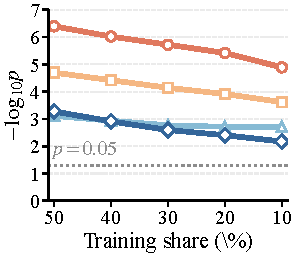
\includegraphics[width=0.82\linewidth]{figure/training_share_bfcl_gpt.pdf}
\caption{BFCL / GPT}
\end{subfigure}\hfill
\begin{subfigure}[t]{0.32\textwidth}
\centering
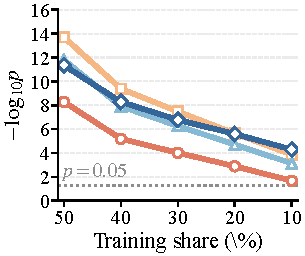
\includegraphics[width=0.82\linewidth]{figure/training_share_swe_bench_gpt.pdf}
\caption{SWE-bench / GPT-OSS-120B}
\end{subfigure}\hfill
\begin{subfigure}[t]{0.32\textwidth}
\centering
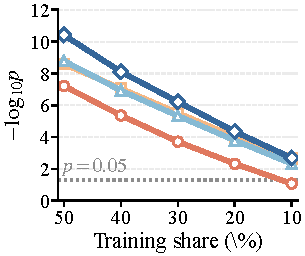
\includegraphics[width=0.82\linewidth]{figure/training_share_telecom_gpt.pdf}
\caption{Telecom / GPT}
\end{subfigure}

\begin{subfigure}[t]{0.32\textwidth}
\centering
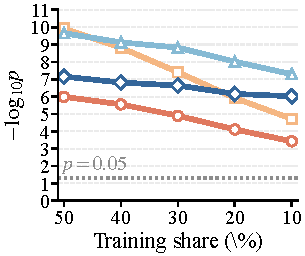
\includegraphics[width=0.82\linewidth]{figure/training_share_bfcl_kimi.pdf}
\caption{BFCL / Kimi}
\end{subfigure}\hfill
\begin{subfigure}[t]{0.32\textwidth}
\centering
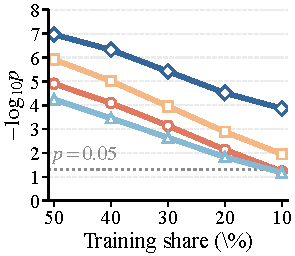
\includegraphics[width=0.82\linewidth]{figure/training_share_swe_bench_kimi.pdf}
\caption{SWE-bench / Kimi-K2.5}
\end{subfigure}\hfill
\begin{subfigure}[t]{0.32\textwidth}
\centering
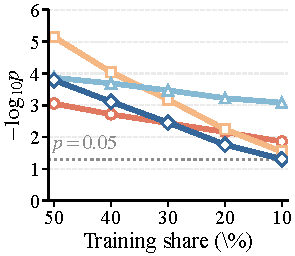
\includegraphics[width=0.82\linewidth]{figure/training_share_telecom_kimi.pdf}
\caption{Telecom / Kimi}
\end{subfigure}
\caption{
Impact of identification accuracy. The horizontal axis denotes the training share and the vertical axis denotes $-\log_{10}p$, where larger values indicate stronger evidence. In (a)--(f), the colored lines and hollow markers denote student models: \textcolor[HTML]{E0795F}{\rule[0.5ex]{0.5em}{1.5pt}\hspace{0.08em}$\circ$\hspace{0.08em}\rule[0.5ex]{0.5em}{1.5pt}} Mistral-24B, \textcolor[HTML]{F5B783}{\rule[0.5ex]{0.5em}{1.5pt}\hspace{0.08em}$\square$\hspace{0.08em}\rule[0.5ex]{0.5em}{1.5pt}} GLM-4.7-Flash, \textcolor[HTML]{86BAD4}{\rule[0.5ex]{0.5em}{1.5pt}\hspace{0.08em}$\triangle$\hspace{0.08em}\rule[0.5ex]{0.5em}{1.5pt}} Qwen3-14B, and \textcolor[HTML]{34669A}{\rule[0.5ex]{0.5em}{1.5pt}\hspace{0.08em}$\diamond$\hspace{0.08em}\rule[0.5ex]{0.5em}{1.5pt}} Qwen3-32B. The \textcolor[HTML]{8C8C8C}{\hdashrule[0.5ex]{1.2em}{1.2pt}{1pt 1.5pt}}  marks $p=0.05$.
}
\label{fig:training-share-sensitivity}
\end{figure*}


\subsection{Supplementary of Robustness}
\label{sec:supplementary-robustness}
\begin{figure*}[!t]
\centering
\begin{subfigure}[t]{\robustnessPanelWidth}
\centering
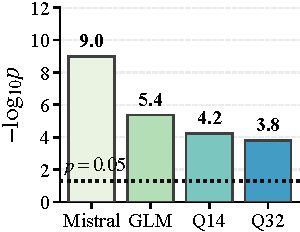
\includegraphics[width=0.72\linewidth]{figure/robustness_data_flooding_plus_bfcl_r1.pdf}
\caption{BFCL: R1}
\end{subfigure}\hfill
\begin{subfigure}[t]{\robustnessPanelWidth}
\centering
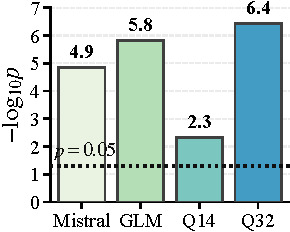
\includegraphics[width=0.72\linewidth]{figure/robustness_data_flooding_plus_bfcl_r2.pdf}
\caption{BFCL: R2}
\end{subfigure}\hfill
\begin{subfigure}[t]{\robustnessPanelWidth}
\centering
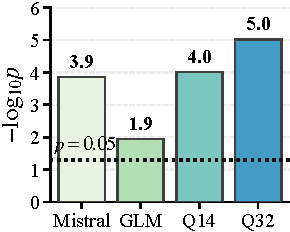
\includegraphics[width=0.72\linewidth]{figure/robustness_data_flooding_plus_bfcl_r3.pdf}
\caption{BFCL: R3}
\end{subfigure}\par
\begin{subfigure}[t]{\robustnessPanelWidth}
\centering
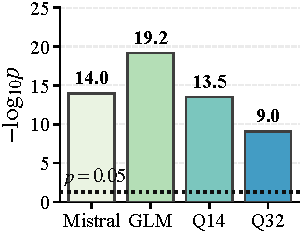
\includegraphics[width=0.72\linewidth]{figure/robustness_data_flooding_plus_swe_bench_r1.pdf}
\caption{SWE-bench: R1}
\end{subfigure}\hfill
\begin{subfigure}[t]{\robustnessPanelWidth}
\centering
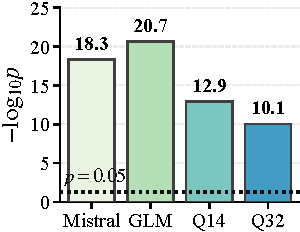
\includegraphics[width=0.72\linewidth]{figure/robustness_data_flooding_plus_swe_bench_r2.pdf}
\caption{SWE-bench: R2}
\end{subfigure}\hfill
\begin{subfigure}[t]{\robustnessPanelWidth}
\centering
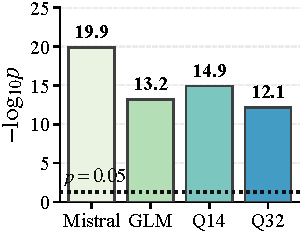
\includegraphics[width=0.72\linewidth]{figure/robustness_data_flooding_plus_swe_bench_r3.pdf}
\caption{SWE-bench: R3}
\end{subfigure}
\caption{Advanced data flooding robustness. The horizontal axis lists the four student models and the vertical axis reports $-\log_{10}p$. In (a)--(f), \robustnessModelLegend. The \textcolor[HTML]{8C8C8C}{\hdashrule[0.5ex]{1.2em}{1.2pt}{1pt 1.5pt}} marks $p=0.05$.}
\label{fig:data-flooding-plus-robustness}
\end{figure*}

\partitle{Advanced data flooding} An attacker may build a diverse training set by collecting solutions to the same tasks from different teacher agents to improve the distilled model's performance~\cite{cui2023ultrafeedback, luo2026agentark}, which also dilutes the watermark signals. To evaluate the robustness of \name{} against this advanced data flooding tactic, we mix the original watermarked dataset $\mathcal{D}_c$ with clean trajectories generated by alternative teacher agents. Specifically, we sequentially introduce clean data from DeepSeek-V4-Flash, MiMo-V2.5, and Qwen3-235B-A22B. In the R1, R2, and R3 settings, we incorporate data from 1, 2, and 3 alternative teachers, resulting in ratios of $1{:}1$, $1{:}2$, and $1{:}3$. Then we use the combined dataset to train the student models and detect their watermarks. We evaluate a total of 24 settings across BFCL and SWE-bench, 3 dilution ratios, and 4 student models. As shown in Figure~\ref{fig:data-flooding-plus-robustness}, \name{} successfully detects every setting. Even under the most challenging R3 setting, all 8 tested student models remain successfully detected.



\partitle{Truncation} Before distillation, an attacker may truncate the trailing tokens of the interaction trajectories to fit the student models' context length limits or to deliberately disrupt potential watermark signals~\cite{kirchenbauer2023watermark}. To evaluate the robustness against this operation, we remove 10\%, 15\%, and 20\% of the tokens from the tail of each watermarked training sequence, and train the student models using these truncated trajectories. We evaluate a total of 24 settings across the BFCL and SWE-bench benchmarks, 3 truncation levels (T10, T15, and T20), and 4 student models. As shown in Figure~\ref{fig:truncation-robustness}, \name{} successfully detects the watermark in every setting. Even under the most aggressive T20 truncation setting, all 8 tested student models remain successfully detected.
\begin{figure*}[!t]
\centering
\begin{subfigure}[t]{\robustnessPanelWidth}
\centering
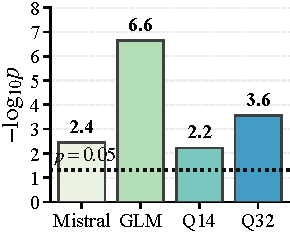
\includegraphics[width=0.72\linewidth]{figure/robustness_truncation_bfcl_t10.pdf}
\caption{BFCL: T10}
\end{subfigure}\hfill
\begin{subfigure}[t]{\robustnessPanelWidth}
\centering
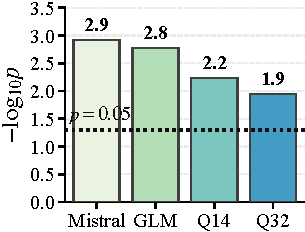
\includegraphics[width=0.72\linewidth]{figure/robustness_truncation_bfcl_t15.pdf}
\caption{BFCL: T15}
\end{subfigure}\hfill
\begin{subfigure}[t]{\robustnessPanelWidth}
\centering
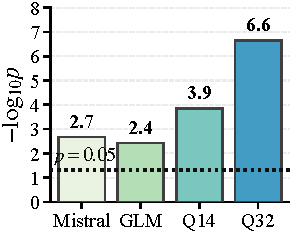
\includegraphics[width=0.72\linewidth]{figure/robustness_truncation_bfcl_t20.pdf}
\caption{BFCL: T20}
\end{subfigure}\par
\begin{subfigure}[t]{\robustnessPanelWidth}
\centering
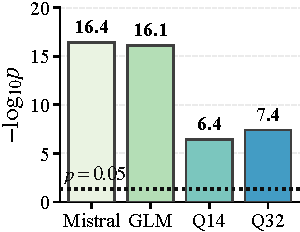
\includegraphics[width=0.72\linewidth]{figure/robustness_truncation_swe_bench_t10.pdf}
\caption{SWE-bench: T10}
\end{subfigure}\hfill
\begin{subfigure}[t]{\robustnessPanelWidth}
\centering
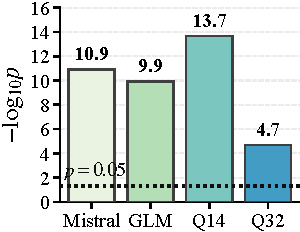
\includegraphics[width=0.72\linewidth]{figure/robustness_truncation_swe_bench_t15.pdf}
\caption{SWE-bench: T15}
\end{subfigure}\hfill
\begin{subfigure}[t]{\robustnessPanelWidth}
\centering
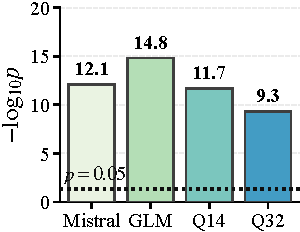
\includegraphics[width=0.72\linewidth]{figure/robustness_truncation_swe_bench_t20.pdf}
\caption{SWE-bench: T20}
\end{subfigure}
\caption{Truncation robustness. The horizontal axis lists the four student models and the vertical axis reports $-\log_{10}p$ . In (a)--(f), \robustnessModelLegend. The \textcolor[HTML]{8C8C8C}{\hdashrule[0.5ex]{1.2em}{1.2pt}{1pt 1.5pt}} marks $p=0.05$.}
\label{fig:truncation-robustness}
\end{figure*}

\begin{table}[!t]
\centering
\caption{Agentwm robustness to data flooding.}
\label{tab:baseline-robustness}
\scriptsize
\setlength{\tabcolsep}{4pt}
\begin{tabular*}{\linewidth}{@{\extracolsep{\fill}}l l | c c@{}}
\noalign{\hrule height 1.5pt}
\textbf{Dataset} & \textbf{Student Model $\mathcal{M}_s$} & \textbf{D1} & \textbf{D5} \\
\hline
\multirow{4}{*}{BFCL} & Mistral-24B & $0/5$ {\color{red}$\times$} & $0/5$ {\color{red}$\times$} \\
& GLM-4.7-Flash & $0/5$ {\color{red}$\times$} & $0/5$ {\color{red}$\times$} \\
& Qwen3-14B & $2/5$ {\color{red}$\times$} & $0/5$ {\color{red}$\times$} \\
& Qwen3-32B & $1/5$ {\color{red}$\times$} & $0/5$ {\color{red}$\times$} \\
\hline
\multirow{4}{*}{SWE-bench} & Mistral-24B & $1/5$ {\color{red}$\times$} & $1/5$ {\color{red}$\times$} \\
& GLM-4.7-Flash & $2/5$ {\color{red}$\times$} & $0/5$ {\color{red}$\times$} \\
& Qwen3-14B & $0/5$ {\color{red}$\times$} & $1/5$ {\color{red}$\times$} \\
& Qwen3-32B & $0/5$ {\color{red}$\times$} & $1/5$ {\color{red}$\times$} \\
\noalign{\hrule height 1.5pt}
\end{tabular*}
\end{table}
\partitle{Baseline robustness} Since Seqwm does not successfully detect distilled students(Table~\ref{tab:baseline-effectiveness}), we focus our robustness evaluation on Agentwm under data flooding (the D1 and D5 settings). To ensure a rigorous comparison, we process the clean standard data to match the initial distribution $P_c$ before mixing it with the watermarked traces. As shown in Table~\ref{tab:baseline-robustness}, all 16 evaluated settings fail to meet Agentwm's $\geq 3/5$ detection threshold. Agentwm encodes its watermark by shifting the tool-variant distribution towards $P_{\mathtt{wm}}$. By flooding the training corpus with clean trajectories calibrated to $P_c$, the overall frequencies are pulled back towards the unwatermarked state. This directly dilutes the artificial distributional signal, resulting in the distilled students not sufficiently reproducing the watermarked patterns for reliable detection.



\section{Discussion on Statistical Test}

\begin{table*}[!t]
\centering
\caption{Comparison of representative anti-distillation methods.}
\label{tab:anti-distillation-comparison}
\begin{threeparttable}
\scriptsize
% Spacing controls: increase/decrease these two values as needed.
\setlength{\tabcolsep}{2.5pt}       % horizontal (column) spacing
\renewcommand{\arraystretch}{1.08}  % vertical (row) spacing

\begin{tabular}{@{}
    >{\raggedright\arraybackslash}p{1.60cm}
    >{\raggedright\arraybackslash}p{2.1cm}
    >{\raggedright\arraybackslash}p{1.70cm}
    >{\centering\arraybackslash}p{0.90cm}
    >{\raggedright\arraybackslash}p{1.8cm}
    >{\centering\arraybackslash}p{0.75cm}
    >{\centering\arraybackslash}p{0.70cm}
    >{\centering\arraybackslash}p{0.75cm}
    >{\raggedright\arraybackslash}p{6.45cm}@{}}
\noalign{\hrule height 1.5pt}
\multirow{2}{1.60cm}{\textbf{Family}} &
\multirow{2}{2.1cm}{\textbf{Shared limits}} &
\multirow{2}{1.70cm}{\textbf{Method}} &
\multirow{2}{0.90cm}{\centering\textbf{Acc.}} &
\multirow{2}{1.8cm}{\textbf{Audit prior}} &
\multicolumn{2}{c}{\textbf{Cost}} &
\multirow{2}{0.75cm}{\centering\textbf{Evid.}} &
\multirow{2}{6.45cm}{\textbf{Main limitation}} \\
\cline{6-7}
& & & & & \textbf{Inject.} & \textbf{Verify} & & \\
\hline

\multirow[c]{5}{1.60cm}{\raggedright Watermarking} &
\multirow[c]{5}{2.15cm}{\raggedright
Limited robustness; additional cost.} &
ADFP &
BB &
Same tasks &
High &
Med. &
Strong &
High cost; sensitive to data dilution; utility loss$^{\star}$.\\

& &
AgentWM &
BB &
Same domain &
Low &
High &
Strong &
Weak cross-model robustness$^{\star}$; sensitive to data dilution$^{\star}$. \\

& &
AgentGuide &
BB &
-- &
Med. &
Low &
Strong &
Does not reliably survive distillation$^{\star}$. \\

& &
SeqWM &
BB &
-- &
Med. &
Low &
Strong &
Does not reliably survive distillation$^{\star}$. \\

\rowcolor{gray!12}
\cellcolor{white} &
\cellcolor{white} &
\textbf{AuxMark} &
\textbf{BB} &
\textbf{Suspected set} &
\textbf{Med.} &
\textbf{Med.} &
\textbf{Strong} &
\textbf{Requires traffic-based screening to select audit candidates.} \\

\hline

\multirow[c]{6}{1.60cm}{\raggedright Fingerprinting} &
\multirow[c]{6}{2.15cm}{\raggedright
No strong evidence of distillation.} &
PoS Templates &
BB/GB &
-- &
-- &
Low &
Weak &
Sensitive to post-training and shared training data. \\

& &
Data-Free KD &
WB &
-- &
-- &
Low &
Weak &
Requires access to the student model's weights. \\

& &
DistillDetect &
GB &
Reference models &
-- &
Low &
Weak &
Requires student logits and calibrated reference models. \\

& &
SCOUT &
BB &
-- &
-- &
Low &
Weak &
Confuses related models; fingerprints may be overwritten. \\

& &
AgentEcho &
BB &
-- &
-- &
High &
Weak &
High AGS across different graph structures.$^{\star}$. \\

& &
Reasoning PF &
BB/GB &
-- &
-- &
Low &
Weak &
High overlap may result from shared solutions or formatting$^{\star}$. \\

\noalign{\hrule height 1.5pt}
\end{tabular}

\begin{tablenotes}[flushleft]
\scriptsize
\item[] BB: black-box access; GB: gray-box access; WB: white-box access.
Low, Med., and High denote relative costs.
Weak denotes indirect or non-distillation-specific evidence; Strong denotes
secret-signal-based attribution. $\star$ indicates a limitation identified by us.
\end{tablenotes}
\end{threeparttable}
\end{table*}


\label{sec:statistical-test-discussion}

\begin{table}[!t]
\centering
\caption{Statistical-unit sensitivity. Entries count settings with an unadjusted one-sided sign-test $p<0.05$; the 15\% training-share row uses the median over 2,000 resamples.}
\label{tab:statistical-unit-sensitivity}
\scriptsize
\setlength{\tabcolsep}{2.5pt}

\begin{tabular*}{\linewidth}{@{\extracolsep{\fill}}p{0.38\linewidth} c c c@{}}
\noalign{\hrule height 1.5pt}

\textbf{Condition} & \textbf{Card-level} & \textbf{Trace-level} & \textbf{Probe-level} \\

\hline

True positives & 24/24 & 24/24 & 24/24 \\
False positives & 0/48 & 0/48 & 3/48 \\
Paraphrasing attack & 8/8 & 7/8 & 8/8 \\
15\% training share & 24/24 & 22/24 & 24/24 \\

\noalign{\hrule height 1.5pt}
\end{tabular*}

\end{table}

To evaluate how the choice of statistical unit affects detection results, we perform the same paired-probe tests at three granularities: card, trace, and probe levels. The card-level test aggregates parameterized probes derived from the same card, the trace-level test further aggregates all cards from the same trajectory, and the probe-level test directly treats each paired probe as an individual statistical unit. As shown in Table~\ref{tab:statistical-unit-sensitivity}, the card- and trace-level tests remain consistent in the main effectiveness evaluation: both achieve 24/24 detections in the true-positive settings and 0/48 significant results in the false-positive settings. Differences mainly appear under more challenging conditions. Trace-level aggregation compresses multiple watermark releases from the same trajectory into a single sign, allowing evidence from different cards to cancel and thereby reducing statistical power and robustness. Consequently, detection decreases from 8/8 to 7/8 under the paraphrasing attack, and from 24/24 to 22/24 at a 15\% training share. In contrast, although probe-level testing shows stronger apparent statistical power, it repeatedly counts parameterized probes that share the same underlying release behavior and context, resulting in 3/48 cases with $p<0.05$ in the false-positive settings. Although none of these cases exceeds the final fullhit-gap threshold and therefore no actual false-positive decision is triggered, the results indicate a higher false-positive risk when probes are counted individually. Based on these observations, we use the card as the primary statistical unit: it avoids repeated counting of the same watermark release event while preserving effective evidence from distinct release events.











\section{A Systematization of Anti-Distillation }
\label{sec:similarity-attribution}









\subsection{Existing Anti-Distillation Methods}


\partitle{Proactive watermarking}
Proactive watermarking embeds signals controlled into teacher outputs, allowing student models to learn and retain these features during distillation. Detecting these signals in student outputs then provides evidence for identifying and verifying distillation. For example, watermarks can be embedded at the token level: ADFP~\cite{xu2026antidistillation} uses a proxy model to estimate how token selection affects watermark learning and adjusts the teacher’s sampling distribution accordingly to improve watermark detectability. Watermarks can also be embedded at the behavioral level: Agentwm~\cite{wang2026protecting} uses functionally equivalent tool paths to embed behavioral watermarks into model execution traces, while Agentguide~\cite{huang2025agent} and SeqWM~\cite{an2026sequential} embed watermarks into model action sequences.

\partitle{Passive fingerprinting}
Passive post-hoc fingerprinting requires no prior embedding of identification signals into teacher outputs. Instead, it retrospectively analyzes similarities between a student model and a candidate teacher to determine whether a distillation relationship exists. Specifically, PoS Templates~\cite{wadhwa2025taught} and SCOUT~\cite{jang2026retrospective} analyze syntactic patterns in generated text; Data-Free KD~\cite{shi2026knowledge} uses model statistics and internal representations for detection; and DistillDetect~\cite{rawat2026reference} compares the likelihood scores assigned to text by the student and reference models. At the behavioral and reasoning levels, AgentEcho~\cite{yang2026agents} examines similarities between tool-calling traces, while Reasoning PF~\cite{panfilov2026stealing} investigates a model’s continuation when private reasoning traces are supplied as prefilled context.


\subsection{Systematic Limitations}
\subsubsection{Overview}
We systematically evaluate representative anti-distillation methods in terms of their cost, evidentiary strength, and primary limitations. As summarized in Table~\ref{tab:anti-distillation-comparison}, the two families exhibit distinct shared limitations. Watermarking methods can provide stronger evidence, but adding and checking watermarks introduces extra cost. Existing watermarks are also not robust and can be weakened by data processing methods such as data dilution. Fingerprinting methods are not enough to prove that unauthorized distillation occurred. Overall, existing methods cannot provide acceptable cost, strong robustness, and reliable evidence at the same time.

\begin{figure*}[!t]
    \centering
    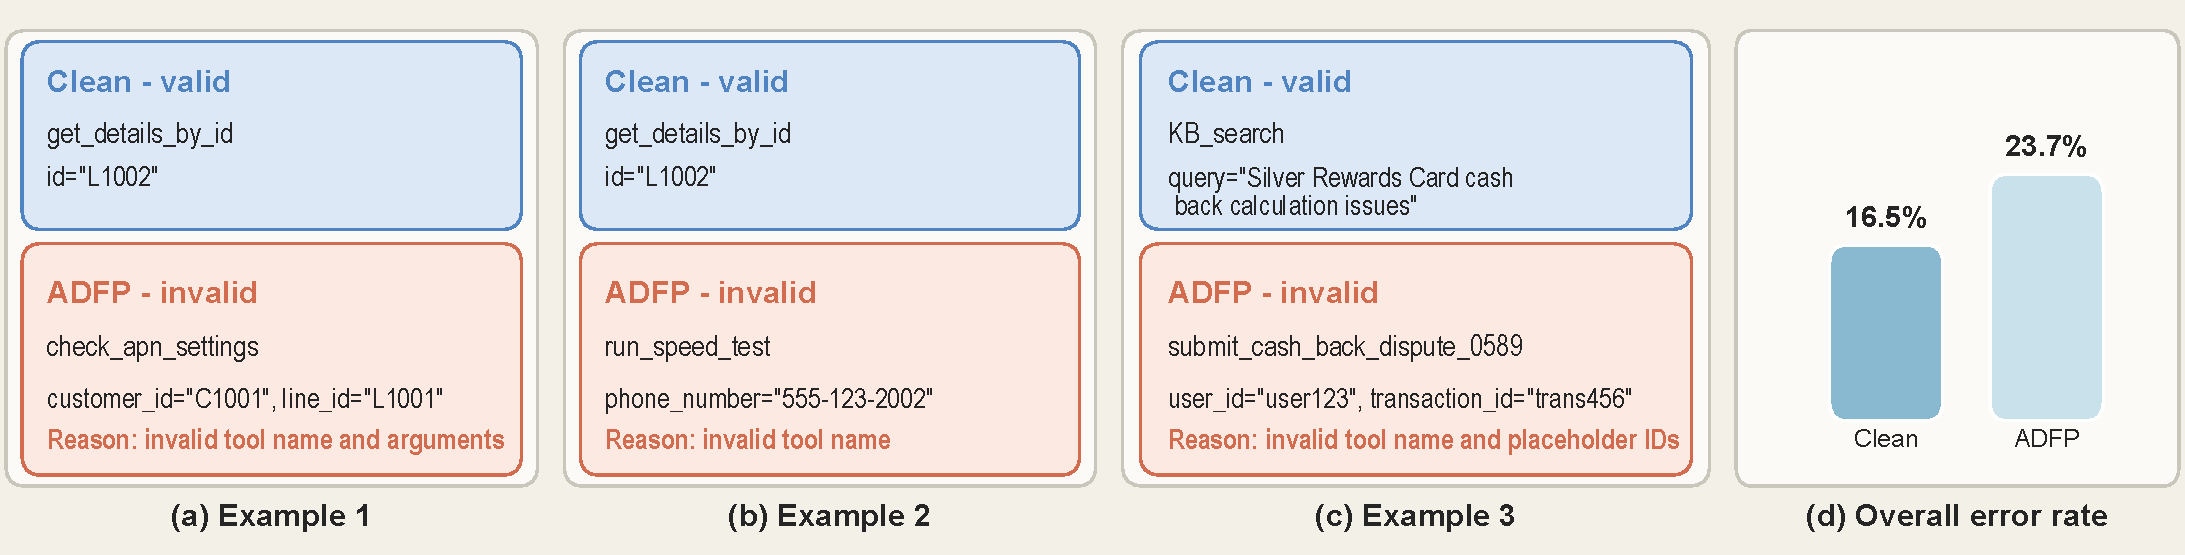
\includegraphics[width=\textwidth]{figure/adfp_agent_utility_failures.pdf}
    \caption{ADFP utility loss. Panels (a)--(c) show three trajectory excerpts,
    each taken from the same-numbered interaction round of the same question.
    The clean trajectory produces a valid tool call, whereas the ADFP trajectory
    invokes a nonexistent tool or uses incorrect arguments. Panel (d) reports
    the overall error rate across all tool calls.}
    \label{fig:adfp-agent-utility}
\end{figure*}

\subsubsection{Limitations of Proactive Watermarking}
Proactive watermarking embeds controlled signals into teacher outputs and can
therefore provide stronger evidence of distillation. However, existing methods
still have limitations in utility, cost, and robustness. ADFP~\cite{xu2026antidistillation} changes the token-sampling process and requires an additional proxy model during decoding. Such token-level changes may corrupt structured outputs in agent settings. We evaluate ADFP with $\lambda=140$ on 20 Tau2 tasks using Qwen3-14B as the teacher and Qwen3-8B as the student. The tool-call error rate increases from $22/133$ ($16.5\%$) in the clean setting
to $31/131$ ($23.7\%$) with ADFP. As shown in Figure~\ref{fig:adfp-agent-utility}, ADFP trajectories may invoke nonexistent tools or produce incorrect arguments. ADFP is also sensitive to data flooding: in the partially fingerprinted data experiment in Section~5.2 and Figure~6 of the original paper, mixing fingerprinted and clean outputs at a 1:1 ratio yields $p>0.05$ in all four unsupervised evaluation settings, so the fingerprint is no longer statistically significant~\cite{xu2026antidistillation}. ADFP is also sensitive to data flooding in Section~5.2 and Figure~6 of the original paper, mixing watermarked data and clean data at a 1:1 ratio yields $p>0.05$ in all four unsupervised evaluation settings, so the fingerprint is no longer statistically significant.

AgentWM~\cite{wang2026protecting} introduces behavioral signals with relatively low embedding cost, but its effectiveness drops greatly when the teacher and
student use different base models. Its signals can also be weakened by
watermark dilution as shown in Table~\ref{tab:baseline-robustness}. AgentGuide~\cite{huang2025agent} and SeqWM~\cite{an2026sequential} require additional watermark embedding or
verification, while their signals may not reliably survive distillation.
As shown by our baseline results in Section~\ref{sec:detection-effectiveness} and Table~\ref{tab:baseline-effectiveness}, AgentWM succeeds only for the GLM-4.7-Flash student, while SeqWM fails to detect any of the tested distilled students. Therefore, existing proactive watermarking methods cannot simultaneously preserve agent utility, remain robust to model and data changes, and keep deployment costs within an acceptable range.


\subsubsection{Limitations of Passive Fingerprinting}
Passive fingerprinting requires no changes to teacher outputs, but its evidence is usually indirect and may not remain stable under model or data changes. PoS Templates~\cite{wadhwa2025taught} relies on syntactic patterns inherited from the teacher, but these patterns may be weakened by further fine-tuning, data augmentation, multi-teacher distillation, or shared training data. Data-Free KD~\cite{shi2026knowledge} requires white-box access to the student model's weights. DistillDetect~\cite{rawat2026reference} relies on student logits and calibrated reference models, making it difficult to use through a standard black-box API. SCOUT~\cite{jang2026retrospective} supports black-box detection, but may confuse related models, and its fingerprints can be overwritten by later training. Therefore, these methods are sensitive to post-training changes and mainly provide indirect similarity-based evidence rather than strong evidence of unauthorized distillation.






\subsection{Vulnerabilities in Token-Level N-gram Matching}
\label{sec:textual-similarity}

\citet{panfilov2026stealing} study visible-answer overlap after prefilling a model's reasoning channel with a short teacher reasoning prefix. Their
Appendix~B.2 evaluates 30 Humanity's Last Exam problems using shared
1-, 2-, and 3-grams against the first 100 tokens of the reference answer,
with best-of-$k$ sampling up to $k=100$. The visible answer is generated
entirely by the target model. Their Figures~11--23 illustrate 13 public
examples with problem statements, teacher reasoning excerpts, and
visible-answer excerpts. Using selected public cases, we test whether
alternative prefixes and shared solution patterns can produce high
overlap with the same teacher reference.

We use a fixed local overlap implementation. For each candidate $a$ and
reference $b$, we tokenize both texts with the same regex tokenizer and
retain up to their first 100 tokens. Let $G_n(x)$ denote the set of distinct
$n$-grams in the retained tokens of $x$. We compute
\begin{equation}
    s_{\mathtt{ngram}}(a,b)
    =
    \frac{\sum_{n=1}^{3}|G_n(a)\cap G_n(b)|}
         {\sum_{n=1}^{3}|G_n(b)|}.
    \label{eq:local-ngram-proxy}
\end{equation}

\partitle{Alternative prefixes and comparisons across model versions}
On the geometry problem in Figure~11 of \citet{panfilov2026stealing},
Kimi-K2.6, which was publicly released before Claude Opus~4.8
\citep{team2025kimi,anthropic2026opus48},
obtains mean/best-of-4 scores of $0.274/0.565$ with the
teacher opening \texttt{This is a known}, compared with $0.373/0.662$
under \texttt{This is an unfamiliar} and $0.250/0.415$ without a prefix.
The best local score of $0.662$ approaches the reported $0.80$ overlap
between prefilled Kimi-K3 and Opus~4.8.
Within this fixed scoring setup, the alternative prefix produces a larger
increase than the authentic prefix across both metrics.
The selected $0.662$ answer shares the opening derivation order $C,F,E,D,B$
with the Opus~4.8 reference, as shown in Figure~\ref{fig:geometry-answer-comparison}.
The sampled Opus~4.6 answers use tables or
different orders; the highest score among these answers is $0.343$ against the
same reference. Thus, this local formatting match is not exclusive to the
teacher prefix or to the sampled Claude-family answers.

\partitle{Convergence on standard solutions}
For the linear differential equation in Figure~13 of
\citet{panfilov2026stealing}, a standard solution uses a $\cosh$ integrating
factor. Without a teacher prefix,
GPT-OSS-120B reaches a mean overlap of $0.500$ and a best-of-4 score of
$0.537$. Kimi-K2.6 similarly scores $0.501$ without a prefix and $0.502$
with the teacher prefix. The unprefilled local scores are numerically close
to the reported $0.50$ overlap between prefilled Kimi-K3 and Opus~4.8.
The unprefilled answer excerpts are shown in Figure~\ref{fig:ode-answer-comparison}.
Our results show that substantial local overlap can arise in standard
solutions with conventional terminology and ordering, while the teacher
prefix adds little in the Kimi-K2.6 comparison.

\partitle{Response steering and sampling}
Visible-answer overlap must also be interpreted in light of how responses
are generated, presented, and selected. In our geometry evaluation of Kimi-K3,
all 20 completions across five prefix
conditions re-derive the solution, and none states the answer within its
first 50 reasoning tokens, unlike the early answer in the reference trace.
Higher visible overlap can therefore coexist with a different observed
reasoning pattern. At the level of answer presentation, even correct
solutions can receive very low scores when little matching text is
available: for the problem in Figure~15 of \citet{panfilov2026stealing},
four correct answers constrained to at most
15 words each score $0.005$. Such sensitivity to presentation also matters
when interpreting best-of-$k$ results, which report the largest overlap
in a sampling pool. Formatting cues can therefore raise the reported score
through occasional high-overlap completions without representing typical
output behavior.
\begin{figure*}[!t]
    \centering
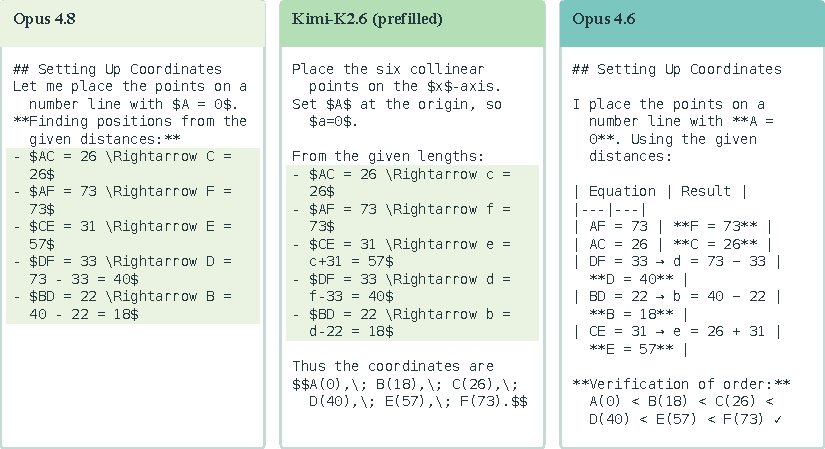
\includegraphics[width=0.72\textwidth]{figure/geometry_answer_comparison.pdf}
    \caption{Excerpts from the original answers to the geometry problem in
    Figure~11 of \citet{panfilov2026stealing}.
    Green shading marks the shared $C,F,E,D,B$ derivation order.
    For each candidate model, we show the highest-overlap answer from four
    samples.}
    \label{fig:geometry-answer-comparison}

    
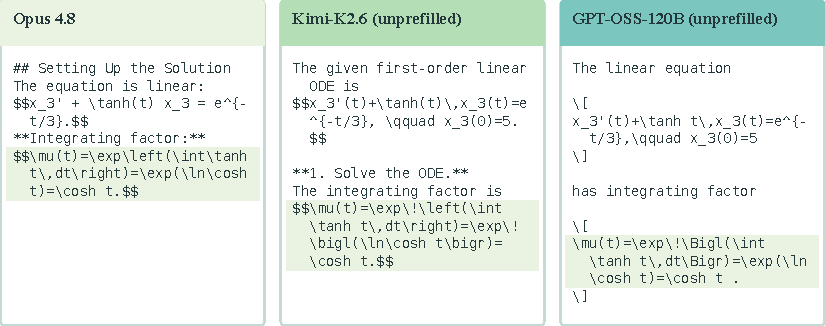
\includegraphics[width=0.72\textwidth]{figure/ode_answer_comparison.pdf}
    \caption{Excerpts from the original answers to the differential-equation
    problem in Figure~13 of \citet{panfilov2026stealing}.
    Green shading marks the shared $\cosh t$ integrating factor.
    Each candidate has the highest reported overlap among four unprefilled
    samples.}
    \label{fig:ode-answer-comparison}
\end{figure*}
\subsection{Vulnerabilities in Agent Execution Graph Similarity}
\label{sec:dependency-ambiguity}
AgentEcho's Action Graph Similarity (AGS) averages optional-tool agreement
$S_{\mathtt{node}}$, sequential-pattern similarity $S_{\mathtt{seq}}$,
and dependency-pattern similarity $S_{\mathtt{dep}}$
\citep{yang2026agents}. Moving from text to tool behavior introduces
structural evidence, but its interpretation depends on which graph
properties the metrics preserve.

\partitle{Scale invariance and structural ambiguity}
For a dependency graph $G$, $S_{\mathtt{dep}}$ compares
$\phi(G)=(r_{\mathtt{reuse}},d_{\mathtt{max}},r_{\mathtt{fanout}})$ by cosine
similarity \citep[Appendix~B.4]{yang2026agents}. These features describe
the fraction of calls after the first that receive dependency inputs,
the longest dependency path, and the fraction of
source nodes with multiple outgoing dependency edges. Cosine similarity
ignores feature-vector magnitude. Consider two graphs with 11 nodes:
one contains a single dependency edge, whereas the other is a complete
10-edge chain. With path length measured in edges,
\begin{equation}
    \phi(G_{\mathtt{single}})=(0.1,1,0),\qquad
    \phi(G_{\mathtt{chain}})=(1,10,0)
    =10\phi(G_{\mathtt{single}}).
    \label{eq:dependency-counterexample}
\end{equation}
Their $S_{\mathtt{dep}}$ is exactly 1 despite large differences in reuse
and dependency depth. Hence, a perfect score does
not guarantee closely matching dependency structures.

\partitle{Evidence from tool trajectories}
We audit 75 trajectories from five models on 15 tasks and compare all
ten model pairs within each task, yielding 150 comparisons.
The mean $S_{\mathtt{dep}}$ is $0.885$,
and 121 comparisons score at least $0.9$. Among these, 53 have dependency
edge counts differing by at least three, and 49 pair a successful
trajectory with a failed one. In \texttt{retail-37}, a failed trajectory
with one dependency edge and a successful trajectory with 12 edges score
$0.991$. We further verify candidate dependency edges with an LLM judge,
using anonymized values and a prompt adapted from the published protocol
\citep[Appendix~B.1]{yang2026agents}.
Both the score and the edge-count discrepancy remain unchanged for this
example.
Thus, near-perfect dependency similarity persists despite substantial
structural differences, even after LLM-based edge verification.

\partitle{Behavioral convergence after reasoning distillation}
\label{sec:reasoning-distillation-convergence}
Inspired by the reference-based formulation of \citet{rawat2026reference},
we measure changes in behavioral similarity relative to the base checkpoint.
We use the Qwen3.5-9B base model as the reference checkpoint and evaluate
its publicly released reasoning-distilled variant.\footnote{Model card:
\href{https://huggingface.co/Jackrong/Qwen3.5-9B-Claude-4.6-Opus-Reasoning-Distilled-v2-GGUF}{Jackrong's
reasoning-distilled Qwen3.5-9B (GGUF)}.}
The model card identifies Claude Opus~4.6 as the teacher.
Our audit of 12,592 publicly available examples from the model card's
listed datasets finds no structured tool trajectories.
We use the same agent harness
and user simulator for 15 $\tau$-bench-style tasks, with one rollout per
model and task. Claude Sonnet~4.5 (thinking), Kimi-K2 (thinking), and
GPT-OSS-120B serve as comparison models.

\begin{table}[!t]
    \centering
    \scriptsize
    \setlength{\tabcolsep}{2pt}
    \resizebox{\columnwidth}{!}{%
    \begin{tabular}{lrrrrrr}
        \hline
        Comparison model & AGS$_{\mathtt{base}}$ & AGS$_{\mathtt{dist}}$
        & $\Delta\mathtt{AGS}$ & $\Delta S_{\mathtt{node}}$
        & $\Delta S_{\mathtt{seq}}$ & $\Delta S_{\mathtt{dep}}$ \\
        \hline
        Claude Sonnet~4.5 (thinking) & 0.549 & 0.709 & +0.160 & $-0.031$ & +0.425 & +0.086 \\
        Kimi-K2 (thinking) & 0.561 & 0.850 & +0.289 & +0.042 & +0.750 & +0.077 \\
        GPT-OSS-120B & 0.584 & 0.770 & +0.186 & $-0.047$ & +0.525 & +0.080 \\
        \hline
    \end{tabular}
    }
    \caption{Changes in AGS and its components after reasoning
    distillation on the same 15 tasks.
    Component values are rounded independently.}
    \label{tab:reasoning-distillation-similarity}
\end{table}

Table~\ref{tab:reasoning-distillation-similarity} shows that AGS increases
toward all three models, alongside a rise in task success from
$4/15$ to $12/15$. The gains are dominated by $S_{\mathtt{seq}}$, which
increases by $0.425$--$0.750$.
In contrast, $S_{\mathtt{dep}}$ increases by $0.077$--$0.086$, while
$S_{\mathtt{node}}$ decreases toward both Claude and GPT-OSS.
Thus, these gains primarily reflect convergence in local execution
statistics and do not uniquely identify teacher-specific tool-use inheritance.

\partitle{Implications for attribution}
These cases expose ambiguity in interpreting high unwatermarked similarity
as evidence of a specific training source. They motivate controls for shared
solutions, response presentation, and general behavioral improvement,
alongside calibrated false-positive rates. Our watermarking framework
provides private verification signals tied to recorded teacher interactions.

\section{Detailed Watermarking Protocols}

\begin{figure*}[!t]
\hrule width \hsize \kern 1mm \hrule width \hsize height 2pt 

\textbf{\name{} Watermark Embedding Protocol}

\hrule

\small
\textbf{Inputs:} Tool schema $\mathcal{F}$, Secret key $k$, Trajectory ID $\mathtt{id}_\tau$, Hyperparameters $(p_0, \Delta p, p_{\mathtt{max}}, B, K)$. \\
\textbf{Outputs:} Watermarked trajectory $\tau$, Private evidence card set $\mathcal{C}_\tau$.


\noindent \textbf{1. Initialization Phase:} 
\begin{itemize}
    \item \textit{System Setup:} 
    \begin{itemize}
        \item Evaluate the tool schema $\mathcal{F}$ using the safety model $\mathcal{M}_{\mathtt{safe}}$ to obtain the valid subset $\mathcal{F}_{\mathtt{safe}}$.
        \item Initialize the dynamic trigger probability $p_1 = p_0$, the remaining budget $b_1 = B$, and an empty evidence set $\mathcal{C}_\tau = \emptyset$.
    \end{itemize}
\end{itemize}

\noindent \textbf{2. Real-Time Embedding Phase:} \\
For each step $t$ immediately following a completed core action $a_{\mathtt{core}}^{t-1}$, the system executes:
\begin{itemize}
    \item \textit{Dynamic Scheduling:}
    \begin{itemize}
        \item Compute a cryptographic hash $u_t = \mathtt{Hash}(k \parallel a \parallel \mathtt{id}_\tau \parallel t) \in [0, 1)$.
        \item If the budget is none ($b_t = 0$) or the condition is not met ($u_t \ge p_t$), skip and failure update.
    \end{itemize}
    
    \item \textit{Candidate Generation \& Scoring:}
    \begin{itemize}
        \item Generate $K$ auxiliary candidates $(t_{\mathtt{aux}}^j, a_{\mathtt{aux}}^j)_{j=1}^K$ using the teacher model $\mathcal{M}_t$ and filter them through the validation mechanism.
        \item For each valid candidate $(t_{\mathtt{aux}}^j, a_{\mathtt{aux}}^j)$, compute the score $S_j$ based on naturalness ($s_{\mathtt{rel}}^j$), logical consistency ($s_{\mathtt{relb}}^j$), and repeatability $s_{\mathtt{relb}}^j$ for the tool pairing $(f_{\mathtt{core}}, f_{\mathtt{aux}}^j)$.
        \item Select the candidate with the highest score as $(t_{\mathtt{aux}}^{\mathtt{best}}, a_{\mathtt{aux}}^{\mathtt{best}})$. If no valid candidates exist, skip to the failure update.
    \end{itemize}

    \item \textit{Injection \& Success Update:}
    \begin{itemize}
        \item Inject $(t_{\mathtt{aux}}^{\mathtt{best}}, a_{\mathtt{aux}}^{\mathtt{best}})$ into the trajectory to receive the auxiliary observation $o_{\mathtt{aux}}^{\mathtt{best}}$.
        \item Reset the probability $p_{t+1} = p_0$ and decrement the budget $b_{t+1} = b_t - 1$.
        \item Increment the historical repeat count for this specific tool pairing $(f_{\mathtt{core}}, f_{\mathtt{aux}}^{\mathtt{best}})$.
        \item Create an evidence card $c_t = (h, t_{\mathtt{core}}^{t-1}, a_{\mathtt{core}}^{t-1}, o_{\mathtt{core}}^{t-1}, f_{\mathtt{aux}}^{\mathtt{best}}, p_{\mathtt{aux}}^{\mathtt{best}})$ and append it to $\mathcal{C}_\tau$.
    \end{itemize}

    \item \textit{Failure/Skip Update (Executed only if no injection occurred):}
    \begin{itemize}
        \item Increase the trigger probability $p_{t+1} = \min\{p_t + \Delta p, p_{\mathtt{max}}\}$ to boost future injection chances, and retain the current budget $b_{t+1} = b_t$.
    \end{itemize}
\end{itemize}

\hrule width \hsize \kern 1mm \hrule width \hsize height 2pt 
\caption{The watermark embedding protocol of \name{}. }
\label{fig:watermark_embedding_protocol}
\end{figure*}

\begin{figure*}[!t]
\hrule width \hsize \kern 1mm \hrule width \hsize height 2pt 

\textbf{\name{} Watermark Detection Protocol}

\hrule

\small
\textbf{Inputs:} Combined evidence pool $\mathcal{C}_{\mathcal{S}}$, Suspect model $\mathcal{M}_s$, Teacher model $\mathcal{M}_t$, Hyperparameters $(p, r, N)$. \\
\textbf{Outputs:} Detection decision $\in \{\mathtt{True}, \mathtt{False}\}$, and the statistical $p\mathtt{-value}$.


\noindent \textbf{1. Probe Construction Phase:} \\
For each evidence card $c_i \in \mathcal{C}_{\mathcal{S}}$, the system executes:
\begin{itemize}
    \item \textit{Paired Probes Generation:}
    \begin{itemize}
        \item Generate up to $N_i$ parameterized variants using card $c_i$ to form the real probe set $p_{\mathtt{real}}^i$.
        \item Construct the corresponding fake probe set $p_{\mathtt{fake}}^i$ by replacing the core action in $p_{\mathtt{real}}^i$ with a semantically altered fake core.
    \end{itemize}
\end{itemize}

\noindent \textbf{2. Evaluation Phase:} \\
For each probe variant $j \in [1, N_i]$ of card $c_i$, the system executes:
\begin{itemize}
    \item \textit{Target Model Query \& Parsing:}
    \begin{itemize}
        \item Submit the real probe $p_{\mathtt{real}, j}^i$ to the suspect model $\mathcal{M}_s$ and parse the output to compute the strict fullhit indicator $h_{i,j}^{\mathtt{real}} \in \{0, 1\}$.
        \item Submit the fake probe $p_{\mathtt{fake}, j}^i$ to the suspect model $\mathcal{M}_s$ and parse the output to compute the strict fullhit indicator $h_{i,j}^{\mathtt{fake}} \in \{0, 1\}$.
    \end{itemize}
\end{itemize}

\noindent \textbf{3. Card-Level Aggregation Phase:} \\
For each card $c_i \in \mathcal{C}_{\mathcal{S}}$, the system executes:
\begin{itemize}
    \item \textit{Hit Rate \& Performance Calculation:}
    \begin{itemize}
        \item Compute the hit rates across all $N_i$ variants: $R_i^{\mathtt{real}} = \frac{1}{N_i} \sum_{j} h_{i,j}^{\mathtt{real}}$ and $R_i^{\mathtt{fake}} = \frac{1}{N_i} \sum_{j} h_{i,j}^{\mathtt{fake}}$.
        \item Calculate the performance difference: $\Delta_i = R_i^{\mathtt{real}} - R_i^{\mathtt{fake}}$.
        \item Tally the results: increment the real win count $w$ if $\Delta_i > 0$, and increment the fake win count $\ell$ if $\Delta_i < 0$ (ties where $\Delta_i = 0$ are excluded).
    \end{itemize}
\end{itemize}

\noindent \textbf{4. Statistical Test \& Decision Phase:} 
\begin{itemize}
    \item \textit{Hypothesis Testing:}
    \begin{itemize}
        \item Compute the one-sided exact sign-test $p\mathtt{-value} = \sum_{k=w}^{w+\ell}\binom{w+\ell}{k}2^{-(w+\ell)}$.
        \item Compute the global mean difference $\Delta_{\mathtt{mean}} = \frac{1}{|\mathcal{C}_{\mathcal{S}}|} \sum_{i} \Delta_i$.
    \end{itemize}
    
    \item \textit{Dual Criteria Check:}
    \begin{itemize}
        \item Output $\mathtt{True}$ (Detection Successful) if both $p\mathtt{-value} < p$ and $\Delta_{\mathtt{mean}} \ge r$ hold. Otherwise, output $\mathtt{False}$.
    \end{itemize}
\end{itemize}

\hrule width \hsize \kern 1mm \hrule width \hsize height 2pt 
\caption{The watermark detection protocol of \name{}.}
\label{fig:watermark_detection_protocol}
\end{figure*}







\end{document}
